
%%%%%%%%%%%%%%%%%%%%%%% file template.tex %%%%%%%%%%%%%%%%%%%%%%%%%
%
% This is a general template file for the LaTeX package SVJour3
% for Springer journals.          Springer Heidelberg 2010/09/16
%
% Copy it to a new file with a new name and use it as the basis
% for your article. Delete % signs as needed.
%
% This template includes a few options for different layouts and
% content for various journals. Please consult a previous issue of
% your journal as needed.
%
%%%%%%%%%%%%%%%%%%%%%%%%%%%%%%%%%%%%%%%%%%%%%%%%%%%%%%%%%%%%%%%%%%%
%
% First comes an example EPS file -- just ignore it and
% proceed on the \documentclass line
% your LaTeX will extract the file if required
\begin{filecontents*}{example.eps}
%\begin{filecontents*}{}
%!PS-Adobe-3.0 EPSF-3.0
%%BoundingBox: 19 19 221 221
%%CreationDate: Mon Sep 29 1997
%%Creator: programmed by hand (JK)
%%EndComments
gsave
newpath
  20 20 moveto
  20 220 lineto
  220 220 lineto
  220 20 lineto
closepath
2 setlinewidth
gsave
  .4 setgray fill
grestore
stroke
grestore
\end{filecontents*}
%
\RequirePackage{fix-cm}
%
%\documentclass{svjour3}                     % onecolumn (standard format)
%\documentclass[smallcondensed]{svjour3}     % onecolumn (ditto)
\documentclass[smallextended]{svjour3}       % onecolumn (second format)
%\documentclass[twocolumn]{svjour3}          % twocolumn
%
\smartqed  % flush right qed marks, e.g. at end of proof
%
\usepackage{graphicx}
\usepackage{lscape}

% PTT
%\usepackage[backend=biber]{biblatex}
%\usepackage[utf8]{inputenc}
%\usepackage[T1]{fontenc}
%
% \usepackage{mathptmx}      % use Times fonts if available on your TeX system
%
% insert here the call for the packages your document requires
%\usepackage{latexsym}
% etc.
%
% please place your own definitions here and don't use \def but
% \newcommand{}{}
%
% Insert the name of "your journal" with
% \journalname{myjournal}
%
\begin{document}

\title{Benchmarking Genetic Programming: A Study Of Generalization Ability Through Noise Models
%\thanks{Grants or other notes
%about the article that should go on the front page should be
%placed here. General acknowledgments should be placed at the end of the article.}
}
%\subtitle{Do you have a subtitle?\\ If so, write it here}

%\titlerunning{Short form of title}        % if too long for running head

\author{ Pham Thi Thuong        \and
        Xuan Hoai Nguyen  \and
        Nam Le 	\and
        Anthony Brabazon
         %etc.
}

%\authorrunning{Short form of author list} % if too long for running head
\institute{Pham Thi Thuong \at
              Thai Nguyen University, Viet Nam \\
              Tel.: ++84-0912-838-646\\
              \email{ptthuong@ictu.edu.vn}           %  \\
%             \emph{Present address:} of F. Author  %  if needed
           \and
            Xuan Hoai Nguyen \at
              AI Academy, Viet Nam \\
              \email: nxhoai@vdspaces.com
           \and
           Nam Le \at
              University College Dublin, Ireland \\
              \email: namlehai90@gmail.com
           \and
           Anthony Brabazon \at
           	  University College Dublin, Ireland  \\
           	  \email: anthony.brabazon@ucd.ie
}

\date{Received: date / Accepted: date}
% The correct dates will be entered by the editor


\maketitle

\begin{abstract}
The objective of this paper is to study the relationship between the overfitting issue and the generalizability of Genetic Programming (GP) when learning noisy training data.
%HOAI - how the relationship is studied in this paper?
Several research questions are addressed such as (1) how noise affects the generalization ability of a GP learning system and what is the relationship between generalization and over-fitting in GP? (2) how to build a suite of benchmarks whose difficulties can be controlled by an over-fitting quantity? (3) how to quantify the overfitting of a benchmark? and (4) how to group these benchmarks into clusters with increasing difficulty based on overfitting levels. We run our experiments on several types of noise along with different magnitudes on the chosen regression benchmarks. Experimental results show that GP is sensitive to noise, and that each type of noise with its corresponding level will have a different effect on the generalizability of GP. A suite of 140 Symbolic Regression problems with noise is created. A new method to quantify the overfitting of problems is proposed. Based on the overfitting of these problems, we group them into 4 problem clusters with increasing overfitting level. It is also suggested to use 140 Symbolic Regression problems in this paper as the benchmarks to study the generalization ability of GP, or its variants, in future research.
\keywords{Genetic Programming \and noise model \and Benchmark Problems \and overfitting}
% \PACS{PACS code1 \and PACS code2 \and more}
% \subclass{MSC code1 \and MSC code2 \and more}
\end{abstract}

\section{Introduction}
\label{Int}
Genetic Programming (GP) was first popularised by Koza \cite {1992Koza} in 1992. Based on Darwinian Evolution by Natural Selection, GP evolves a population of solutions to problems \cite{2008Poli}. GP has been shown to be a powerful enough problem-solver, and has been claimed to be one of the Machine Learning (ML) techniques (\cite{2008Poli}). \par

In Machine Learning, generalization and over-fitting are undoubtedly two amongst the most important issues. They can be seen as the two sides of the same coin and should be addressed simultaneously. There are a number of studies which analyse these issues in GP such as \cite{Fit2013}\cite{Goncalves2012}\cite{Goncalves2013}\cite{Hie2014}\cite{Hien2012}\cite{Uy2010}\cite{2014Uy}\cite{lu2018genetic}\cite{kurtoglu2017fiber}\cite{la2018multidimensional}\cite{haeri2017statistical} to name but a few. However, most of them do not have a systematic way to choose testing problems. Moreover, theoretically, “No free lunch” (NFL) theorem tells us that no algorithm can perform well on all classes of learning problem \cite{1996David}. In practice, it has been advocated in the field of statistics, machine learning, and data science that the common task frame work (CTF) should be adopted to advance these fields \cite{liberman2009,Donoho2017}. In CTF it is necessary to have a suite of benchmarks (called common task), ideally, with different level of difficulties, so that different methods could be tested and compared, even in the form of competitions. The UCI repository and Kaggle are examples of CTF in the fields of Machine Learning and Data Science. The CTF has been utilized in IEEE World Congress on Evolutionary Computation (CEC) for a number of years in the form of various competitions (http://www.ecomp.poli.br/~wcci2018/competitions/). However, there has been no such competition (in the spirit of CTF) for GP.
Thus, it is necessary to have a set of benchmarks with various levels of difficulty with regard to generalization ability of GP. They make it easier for researchers to study how good GP is in terms of generalization (and overfitting), and whether GP can be scalable over a wide range of problems with different complexities. They also facilitate the comparison and reproducibility of various research on the improvements of GP generalization/overfitting, and consequently, help to advance the field of GP.
To the best of our knowledge, there has never been any benchmark for studying generalization and overfitting issues in GP with such characteristics. Therefore, the first target of this paper is to build such a suite of benchmarks, within the domain of symbolic regression. These benchmarks are also grouped into different clusters whose levels of difficulty are controlled by the amount of over-fitting. \par

One reason of being overfitted is the problem of noise in real-world training data \cite{1999Liu}. Several noise models with various types and levels have been proposed to simulate noise in the real-world as close as possible, making learning machines easier to be overfitted. It has also been shown that the different types and levels of noise affect the generalization ability of the learner in different ways (\cite{1994Mark}\cite{1996Hic}\cite{2003Eli}\cite{1999Carla}\cite{2007Daz}\cite{2010Dav}\cite{2011Nic}\cite{2012Loh}\cite{2014Fré})\cite{silva2017semi}\cite{gonccalves2017exploration}. Therefore, the second goal of this paper is to study how noise affects the generalization ability or overfitting of a GP learner. 
%HOAI - there has been some studies on GP symbolic regression with presence of noise (like Paris et al.) but these researched have been limited to single noise model (noise on X). We should add one or two sentences about this!

The contributions of this paper are summarized as follows:
\begin{itemize}
\item Propose a new method to quantify overfitting in GP. This is the priority of this paper. %It is the base for controlling the difficult of benchmark by over-fitting. Because the measure \textquotedblleft the amount of over fit\textquotedblright proposed by Vanneschi usually use in GP has a few limits (see the section \ref{Qua}). So, we propose the new method to improve these limits.
%\item Survey some noise models in Machine Learning and investigate the impacts of noise to over-fitted and generalization ability of solutions in GP.
\item Construct 140 symbolic regression benchmarks by utilizing different noise models, which are grouped into clusters by increasing levels of difficulty, to study generalization and overfitting issues in GP as a learning machine.
\end{itemize} \par

The remainder of this paper is organized as follows. In section \ref{Bac}, we briefly present a survey of GP benchmarks, noise models in Machine Learning, and some issues on how to quantify the overfitting of solutions in GP.  The next section describes several noise configurations used for experiments in this study; a new method to quantify the over-fitting of a problem is also presented in the section \ref{Ane}. Experimental settings are presented in section \ref{Exp}, then results and the discussions are given in section \ref{Res}, and finally section \ref{Con} concludes the paper and gives some proposals for future work.
\section{Background and related works}
\label{Bac}
\subsection {GP benchmarks}
\label{GPb}

Building a set of benchmarks with different difficulties has been recently received much attention from researchers in GP \cite{2012James}, \cite{2015Mig}. It has been said that devising a good benchmark suite would be recognized as an important issue for the next ten years of GP \cite{2010O'Neill}. \par

In \cite {2012James}, the authors presented a list of symbolic regression functions aiming at collecting opinions of GP community. After that, other researchers in \cite{David2013} presented the results of a community survey regarding this list. In \cite{2012James}, the authors introduced some benchmark criteria and listed a suit of problem satisfying these criteria. The way to determine the difficulty of a specific problem has also been proposed in \cite{2012James}, but mainly limited to structural complexity (E.g. The Royal Tree problem, Order and Majority, ... their difficulty can be changed by modifying some parameter values while Boolean problems are scalable because they are self-contained, no requiring external data-set or domain knowledge). In \cite{2014John}, John  and his colleagues suggested that benchmarks should not be selected arbitrarily, but instead should be drawn from an underlying probability distribution that must reflect the problem instances in which the algorithm is likely to be applied to in the real-world. However, these authors did not show how to quantify the difficulty level of a problem. Michael O’Neill and his colleagues in \cite{2010O'Neill} identified the problem difficulty that relates not only to the representation of the solution, but also to the choice of genetic operators and fitness functions.  Fitness landscape can also be helpful to understand the difficulty of a problem \cite{2002Stadle}\cite{1932Wri}. With this in mind, the authors in \cite{2004Vanneschi}\cite{2005Vanneschi} introduced two measurements of the problem hardness for GP, based on the concept of fitness landscape: fitness-distance correlation (FDC) and negative slope coefficient (NSC). The NSC was showed to correctly quantify the difficulty of some GP benchmarks and  real-life problems \cite{2006Vanneschi}. However such fitness based measurements are related to search difficulty rather an generalization difficulty of GP. %The dissimilarity measurement proposed in \cite{2005Gustafson} is another method, which calculates the probability of correctly applying the operator once. Clíodhna Tuite and and colleagues explore for a design of a dynamic benchmark for symbolic regression, based on semantic distance between evaluated functions \cite{2013Tuite}. \par

Recently, Miguel Nicolau and his colleagues showed seven issues concerning the design of symbolic regression benchmarks and provided a set of guidelines to scrutinize these functions \cite{2015Mig}. In addition, they also pointed out that the size of the data set can affect the distribution of response variable and it also can be used to control the difficulty of the problem. It was suggested that larger samples tend to lead to better test performance of the learned model \cite{2015Mig}. In other words, the smaller size of the training set, the more difficult the problem to learn. However, in practice, training data might not be enough that the experimenter could design multiple training sets with different sizes. \par
Thomas Helmuth and Lee Spector presented a suite of 29 benchmarks for GP \cite{Thomas2015}, which are selected from introductory computer science programming problems. These benchmarks vary in difficulty and can be helpful to assessing the capabilities of GP in program synthesis tasks. \par

Most recently, Patryk and his colleagues in \cite{orzechowski2018we} used a set of 94 different real-world regression problems collected from 
Penn Machine Learning Benchmark repository for his research. However, in this research, he only focuses on ranking the performance of the algorithms learned on these problems, rather than sorting these problems based on their difficult levels. Building a suit of symbolic regression problems that can be controlled by their difficult levels is still a open issue.

In short, researchers on the topic of overfitting and generalization in GP mainly focus on questions as follows: how to develop a set of benchmarks for GP and how to determine the difficulty of the problem. There are not quite yet a  benchmark whose difficulties can be compared by over-fitting, in order to study the generalization ability of GP as a learning machine. Therefore, in this paper we build such a benchmark suite by adding noise systematically.

\subsection {Noise models in ML and GP}
\label{Noi}
In this section, we introduce a number of noise models used  in Machine Learning and in GP. Then, we choose one from them for our experiments and explain why we choose it. \par

Two main sources of noise are depicted in \cite{2010Dav}: (1) the erroneous measurement of sensors; (2) the random error created when gathering data or processing in batch. The author also described three characteristics of noise generating process as follows: (1) the distribution of noise: noise is often drawn randomly, especially under a Gaussian distribution; (2) where the noise is introduced: noise can be found in four situations as shown in the Table \ref{tab:CaseOfNoise}; (3) the magnitude of the generated noise values, which is often relative to each variable domain.\par

In \cite{1994Mark}, Mark introduced a model to add noise into state variables in Reinforcement Learning as follows: Assume the noise level was set to k\%, then the state value at the next time step  would be $x + random (-x*k,x*k) + random(-0.0001,0.0001)$, where $x$ is the value at current time step. Adding noise is simply done by this model. However, it was shown to be naive and does not fully reflect characteristics of the noise \cite{1994Mark}. A further improved noise model was also introduced by the same author, and  used in \cite{2003Eli}, in which the two following assumptions are set to be true for all data sets: (1) the variables of the data set (both independent and the dependent) are normally distributed; (2) noise is randomly distributed and independent from the data. Based on these assumptions, noise is generated as follows: \par

For every case ($y_{i}$, $x_{i}$) in the data set $L$: The pair ($y_{i}$, $x_{i}$) of the dependent variable $Y$ and the matrix of independent variables $X$ is substituted by another pair ($y_{i}^{'}$, $x_{i}^{'}$) by a probability $n$, where $n$ also indicates the noise level. The new pair is calculated by the following formula:

$$ x_{ij}^{'} = \left\{ \begin{array}{lll}
x_{ij}+\sigma_{x_{j}}z_{j} & if & p_{ij}\geq n ;\\
x_{ij} & if & p_{ij} \le n .\end{array} \right.
y_{i}^{'} = \left\{ \begin{array}{lll}
y_{i}+\sigma_{y}z_{j} &  if & p_{ij}\geq n ;\\
y_{i} &if &p_{ij} \le n .\end{array} \right. $$
$z_{ij} =norminv(p_{ij}),j\in [1,..,k]$ \par

where: $\sigma_{x_{j}}$ is the standard deviation of $x_{j}$; $z_{j}$ is a  normally distributed random variable and is calculated by the inverse function of the density-probability of the normal distribution for $p_{ij}$, with mean zero and unit standard deviation; $p_{ij} \in (0, 1)$ is a probability variable produced by a random value generator following a uniform distribution. This noise model was also used in \cite{miranda2017noisy} to generate 165 datasets with 11 different levels of noise, to study the effect of noise to the leaning ability of Geometric Semantic Genetic Programming (GSGP). However, in this research, the authors only focused on noise in the output variable of problems, the input variables were not considered to be noisy.

In many cases, the assumption that variables are generated by a normal distribution is not satisfied. In \cite{2010Dav} David and his colleagues described how to generate artificial noise (without any normal distribution assumption) as follows: for each variable $x$, repeat $N*k$ times the following four steps: (1) Randomly generate a value $R_{x}$ under a Gaussian distribution centered around $x$; (2). Uniformly choose an index $i$ between $1$ and $N$, then pick $R_{i}$; (3) Check if $R_{i}$ has been chosen previously or not. If it has been, return to Step 2; (4) Assign $R_{x}$ to $R_{i}$. Where, the magnitude of noise lies between $min$ and $max$ of the corresponding variable, $k$ is a noise level, $n$ is the size of data set for the data set. This model assumes that noise is still under a Gaussian distribution which is not an unusual assumption used in noise models. This is the noise model widely used in Machine Learning algorithms \cite{2010Dav}. Thus, in this paper we use this noise model for our experiments.
% HOAI - this 4 step algorithm should be presented as a flow graph 

\par
\begin{table}
% table caption is above the table
\caption{Possible situations of noise in data sets}
\label{tab:CaseOfNoise}       % Give a unique label
% For LaTeX tables use
\begin{tabular}{ll}
\hline\noalign{\smallskip}
Input data & Output \\
\noalign{\smallskip}\hline\noalign{\smallskip}
Noise in train & Noise in test \\
Noise in test & \\
Noise in train and test & \\
\noalign{\smallskip}\hline
\end{tabular}
\end{table}


\subsection {Quantifying overfitting in GP}
\label{Qua} 

The overfitting issue can be encountered in almost all supervised Machine Learning schemes \cite{1996Mitchell}. This is one of the main causes of losing the generalization power of solutions. To study these issues, at first, it is necessary to have a measurement to quantify over-fitting of problems. In Machine Learning, there has been some research introducing the formula to quantify the amount of overfitting of solutions, such as \cite{2008Trevor}\cite{Marcel}\cite{copas1983regression}\cite{bilger2015measuring}. However, there has been a little work on this issue in GP (as an iterative learner with many generations for each training run). \par

In GP, Silva and colleagues \cite{2010Vanneschi} proposed  a method to quantify overfitting at a given generation $g$ ($overfit(g)$) by the pseudocode shown in the algorithm 1, where, $btp$ (best test point) represents the best test fitness reached until the current generation, excluding the generations (usually at the beginning of the run) in which the best individual on the training set has a better test than training fitness; $tbtp$ (training at best test point) is the training fitness of the individual that has test fitness equal to $btp$ ; $training\_fit(g)$ is a function that returns the best training fitness in the population at generation $g$; $test\_fit(g)$ returns the test fitness of the best individual at generation $g$.

\begin{table}
\begin{tabular}{lllllllllll}
\multicolumn{11}{l}{\textbf{Algorithm 1}: The overfitting measure \cite{2010Vanneschi}} \\
\multicolumn{1}{l|}{} & \multicolumn{10}{l}{$overfit(0) = 0$} \\
\multicolumn{1}{l|}{} & \multicolumn{10}{l}{$btp = test\_fit(0)$} \\
\multicolumn{1}{l|}{} & \multicolumn{10}{l}{$tbtp = training\_fit(0)$} \\
\multicolumn{1}{l|}{} & \multicolumn{10}{l}{\textbf{for each } $generation$ $g>0$ } \\
\multicolumn{1}{l|}{} & \multicolumn{1}{l|}{} & \multicolumn{9}{l}{  \textbf{if} $(training\_fit(g) > test\_fit(g))$} \\
\multicolumn{1}{l|}{} & \multicolumn{1}{l|}{} & \multicolumn{1}{l|}{} & \multicolumn{8}{l}{$overfit(i)= 0$} \\
\multicolumn{1}{l|}{} & \multicolumn{1}{l|}{} & \multicolumn{9}{l}{   \textbf{else}} \\
\multicolumn{1}{l|}{} & \multicolumn{1}{l|}{} & \multicolumn{1}{l|}{} & \multicolumn{8}{l}{\textbf{if} $(test\_fit(g) < btp)$}  \\
\multicolumn{1}{l|}{} & \multicolumn{1}{l|}{} & \multicolumn{1}{l|}{} & \multicolumn{1}{l|}{} & \multicolumn{7}{l}{$overfit(g)= 0$} \\
\multicolumn{1}{l|}{} & \multicolumn{1}{l|}{} & \multicolumn{1}{l|}{} & \multicolumn{1}{l|}{} & \multicolumn{7}{l}{$btp = test\_fit(g)$} \\
\multicolumn{1}{l|}{} & \multicolumn{1}{l|}{} & \multicolumn{1}{l|}{} & \multicolumn{1}{l|}{} & \multicolumn{7}{l}{$tbtp = training\_fit(g)$} \\
\multicolumn{1}{l|}{} & \multicolumn{1}{l|}{} & \multicolumn{1}{l|}{} & \multicolumn{8}{l}{ \textbf{else} } \\
\multicolumn{1}{l|}{} & \multicolumn{1}{l|}{} & \multicolumn{1}{l|}{} & \multicolumn{1}{l|}{} & \multicolumn{7}{l}{ $overfit(g) = |training\_fit(g) - test\_fit(g)| - |tbtp-btp| $} \\
\multicolumn{1}{l|}{} & \multicolumn{1}{l|}{} & \multicolumn{1}{l|}{} & \multicolumn{8}{l}{\textbf{endif}} \\
\multicolumn{1}{l|}{} & \multicolumn{1}{l|}{} & \multicolumn{9}{l}{\textbf{endif}} \\
\multicolumn{1}{l|}{} & \multicolumn{10}{l}{\textbf{endfor}} \\

\end{tabular}
\end{table} 

Intuitively and experimentally, we find out some issues arising from this formula. The details of these issues and the new overfitting measures will be presented in section \ref{Ane}.

\section{Methods}
\label{Met}
\subsection{Generating noise}
\label{Gen}
Noise can be presented at the training set, or the testing set, or both. It has been shown that noise in the training data set accounts for most difficulties to learners \cite{2011Nic}. Therefore, in this paper we focus on learning problems in which noise is added into training instances only. As presented in section \ref{Noi}, we adopt the noise model introduced in \cite{2010Dav} and just add noise into the original training set while the testing set is unchanged.  Noise is added to independent variables x (noise type x), or response variable y (noise type y), and or both x \& y (noise type xy), with corresponding noise levels: 0\% (free Noise), 10\% (low noise), 30\% (medium noise) and 50\% (high Noise). The noise configuration employed in this paper is presented below:\par

\begin{itemize}
\item \textit{F: training set with 0 \% noise (the original data set)}
\item \textit{Lx: 10\% noise x in the training data}
\item \textit{Mx: 30\% noise x in the training data}
\item \textit{Hx: 50\% noise x in the training data}
\item \textit{Ly: 10\% noise y in the training data}
\item \textit{My: 30\% noise y in the training data}
\item \textit{Hy: 50\% noise y in the training data}
\item \textit{Lxy: 10\% noise xy in the training data}
\item \textit{Mxy: 30\% noise xy in the training data}
\item \textit{Hxy: 50\% noise xy in the training data}
\end{itemize} \par

A point worth noting here is that the distribution of independent variables x and response variable y is not significantly changed after having noise added. Table \ref{tab:pvalueNoise} shows p-values obtained by comparing the difference in x, y before and after having noise added using Mann Whitney U Test use, with 95\% confidence. %All $p value \ge 0.05$ for all variables of all problems) \par

%\begin{landscape}
\begin{table}
% table caption is above the table
\caption{p values obtained by comparing the difference in x, y to x, y added noise using Mann Whitney U Test use, with 95\% confidence}
\label{tab:pvalueNoise}       % Give a unique label
% For LaTeX tables use
\begin{tabular}{lllllllllll}
\hline\noalign{\smallskip}
Problem & Var & Lx & Mx & Hx & Ly & My & Hy & Lxy & Mxy & Hxy \\
\noalign{\smallskip}\hline\noalign{\smallskip}
Kei10 & x1 & 0.951 & 0.80 & 0.48 &  &  &  & 0.79 & 0.96 & 0.48 \\
& x2 & 0.92 & 0.66 & 0.37 & & & & 0.65 & 0.53 & 0.34 \\
& y &  & & & 0.65 & 0.72 & 0.57 & 0.99 & 0.69 & 0.75 \\
Kei11 & x1 & 0.97 & 0.35 & 0.47 & &  &  & 0.70 & 0.79 & 0.47 \\
& x2 & 0.78 & 0.89 & 0.19 &  &  & & 0.95 & 0.98 & 0.19 \\
& y & & & & 0.65 & 0.70 & 0.45 & 0.95 & 0.81 & 0.62 \\
Kei12 & x1 & 0.98 & 0.82 & 0.73 & & & & 0.82 & 0.70 & 0.85 \\
& x2 & 0.82 & 0.96 & 0.47 &  &  & & 0.83 & 0.55 & 0.47 \\
& y & & & & 0.86 & 0.85 & 0.92 & 0.69 & 0.96 & 0.28 \\
Kei13 & x1 & 0.67 & 0.49 & 0.62 & & & & 0.78 & 0.63 & 0.61 \\
& x2 & 0.62 & 0.79 & 0.24 & & & & 0.90 & 0.75 & 0.24 \\
& y & & & & 0.47 & 0.60 & 0.88 & 0.91 & 0.68 & 0.82 \\
Kei14 & x1 & 0.83 & 0.42 & 0.86 & & & & 0.76 & 0.94 & 0.86 \\
& x2 & 0.50 & 0.68 & 0.25 & & & & 0.98 & 0.55 & 0.25 \\
& y & & & & 0.92 & 0.77 & 0.84 & 0.85 & 0.39 & 0.55 \\
Kei15 & x1 & 0.89 & 0.70 & 0.99 & & & & 0.66 & 0.76 & 0.99 \\
& x2 & 0.65 & 0.80 & 0.47 & & & & 0.72 & 0.69 & 0.47 \\
& y & & & & 0.86 & 0.61 & 0.61 & 0.85 & 0.59 & 0.15 \\
Vla1 & x1 & 0.86 & 0.76 & 0.77 & & & & 0.84 & 0.93 & 0.77 \\
& x2 & 0.53 & 0.95 & 0.34 & & & & 0.53 & 0.95 & 0.34 \\
& y & & & & 0.73 & 0.68 & 0.93 & 0.75 & 0.23 & 0.89 \\
Vla5 & x1 & 0.95 & 0.43 & 0.80 & & & & 0.75 & 0.95 & 0.80 \\
& x2 & 0.94 & 0.63 & 0.39 & & & & 0.98 & 0.89 & 0.39 \\
& x3 & 0.95 & 0.96 & 0.59 & & & & 0.92 & 0.91 & 0.59 \\
& y & & & & 0.83 & 0.49 & 0.63 & 0.78 & 0.56 & 0.68 \\
Vla6 & x1 & 0.80 & 0.35 & 0.98 & & & & 0.95 & 0.52 & 0.982 \\
& x2 & 0.86 & 0.71 & 0.22 & & & & 0.87 & 0.52 & 0.22 \\
& y & & & & 0.59 & 0.82 & 0.80 & 0.83 & 0.69 & 0.98 \\
Vla8 & x1 & 0.98 & 0.89 & 0.74 & & & & 0.86 & 0.86 & 0.739 \\
& x2 & 0.68 & 0.94 & 0.48 &  & & & 0.57 & 0.72 & 0.48 \\
& y & & & & 0.60 & 0.94 & 0.48 & 0.87 & 0.26 & 0.74 \\
Nguyen\_1 & x & 0.89 & 0.98 & 0.64 & & & & 0.85 & 0.81 & 0.64 \\
& y & & &  & 0.82 & 0.85 & 0.83 & 0.76 & 0.96 & 0.78 \\
Nguyen\_2 & x & 0.72 & 0.98 & 0.37 & & & & 0.95 & 0.87 & 0.375 \\
& y & & & & 0.75 & 0.63 & 0.80 & 0.51 & 0.52 & 0.79 \\
Nguyen\_3 & x & 0.91 & 0.57 & 0.30 & & & & 0.90 & 0.38 & 0.305 \\
& y & &  & & 0.82 & 0.70 & 0.88 & 0.47 & 0.77 & 0.60 \\
Nguyen\_4 & x & 0.68 & 0.56 & 0.72 & & & & & 0.93 & 0.72 \\
& y & & & & 0.80 & 0.74 & 0.52 & 0.64 & 0.89 & 0.36 \\
\hline
\end{tabular}
\end{table}
%\end{landscape}


\subsection{A new method to quantify the over-fitting}
\label{Ane}
\subsubsection{The issues of the overfitting measurement in \cite{2010Vanneschi} }
As mentioned in section \ref{Qua}, the overfitting measurement proposed in \cite{2010Vanneschi} has some weaknesses. Given a learner (e.g., GP); a training data set (e.g., s); a generation obtained while learning (e.g., $g$), that overfitting measurement only starts calculating the overfitting at $g$ when the condition (1) $training\_fit(g) \le test\_fit(g)$ is true. Therefore, this leads to some issues as follows: 

\begin{enumerate}
\item \textit{The first issue is that measurement ignores some generations in which the learner is overfitted}\\

It is noted that if overfitting arises at a generation before the condition (1) is true, then the measurement by Silva does not calculate the amount of overfitting (OV) at that generation. %This also means that it will ignores the calculation the OV at all overfitted gererations if this condition is always fail. 
To understand this issue visually, we depict the empirical results with some counterexample cases as shown in Figure \ref{fig:issue1}. In this Figure, it can be seen that overfitting arises in most cases of problems. However, the overfit(g) values return by Silva's measurement is always set to 0 at every generation g, except the case of problem Nguyen4.Ly. Even with this problem, Silva's measurement only calculates the overfitting at generations from 66 and ignores the overfitted generations before that. The corresponding overfitting (rounded) at generations from 66 to 151 of this problem are: \\

\textit{0.00; 0.01; 0.01; 0.02; 0.03; 0.03; 0.04; 0.03;
0.02; 0.05; 0.05; 0.05; 0.06; \\0.06; 0.06; 
0.07; 0.06; 0.07; 0.07; 0.08; 0.08; 0.08; 0.08; 0.08; 0.09; 0.09;\\ 0.09; 0.10; 0.10; 0.10; 0.11; 0.11; 0.11; 0.11; 0.12; 0.12; 0.11; 0.11; 0.12;\\
0.12; 0.12; 0.13; 0.13; 0.13; 0.13; 0.14; 0.14; 0.14; 0.15; 0.15; 0.15; 0.15;\\
0.15; 0.15; 0.15; 0.15; 0.16; 0.17; 0.17; 0.17; 0.17; 0.17; 0.18; 0.18; 0.18;\\
0.18; 0.18; 0.18; 0.18; 0.19; 0.19; 0.19; 0.19; 0.19; 0.19; 
0.19; 0.19; 0.19; \\
0.19; 0.20; 0.20; 0.20; 0.20; 0.20; 0.20; 0.20 \\
}
% For one-column wide figures use
\begin{figure}
% Use the relevant command to insert your figure file.
% For example, with the graphicx package use
\centering
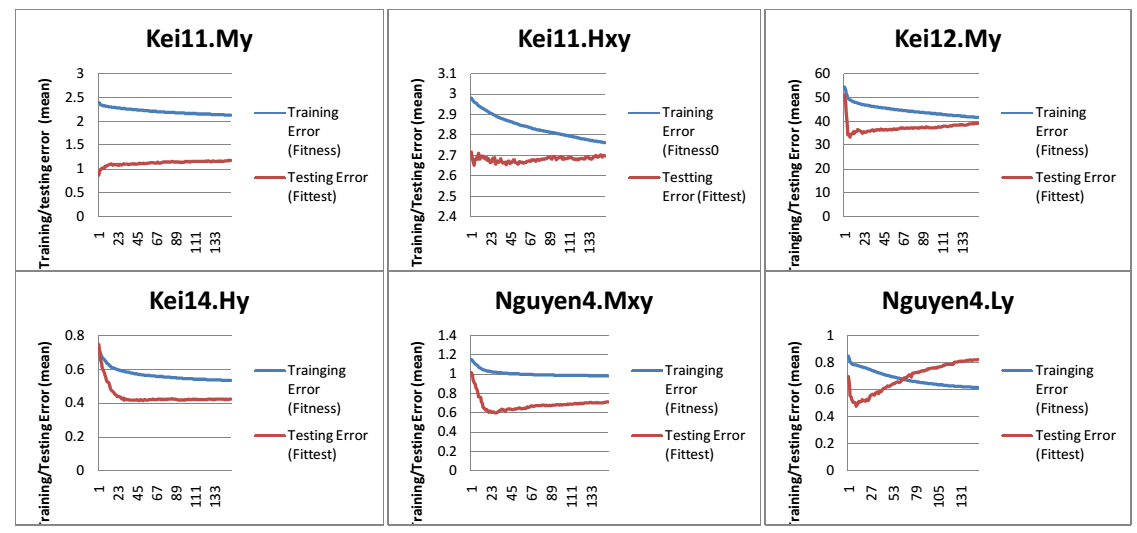
\includegraphics[scale=0.4]{Figures/Fig3_1.png}
% figure caption is below the figure
\caption{Some cases arise the first issues with the overfitting measurement proposed by Silva and colleagues.}
\label{fig:issue1}       % Give a unique label
\end{figure}


\item \textit{The second issue is the detection of the best test point (btp)} \\ 
Correctly detecting the best test point will help us in finding the generation where the overfitting issue starts to occur. This is very useful, especially when we want to study the early stopping of GP learners. However, by looking at the Nguyen4.Ly problem as shown in the Figure \ref{fig:issue2.1} we see that this overfitting measure also fails to capture the best test point correctly. The actual best test point ($btp_{actual}$) found (at the $66^{th}$generation) is different from the expected best test point ($btp_{expected}$) (at generation $11^{th}$). The same issue (blocked while finding the $btp_{expected}$) caused by the condition (1) of this measure also occurs in cases as shown in the Figure \ref{fig:issue2.2}.

% For one-column wide figures use
\begin{figure}
% Use the relevant command to insert your figure file.
% For example, with the graphicx package use
\centering
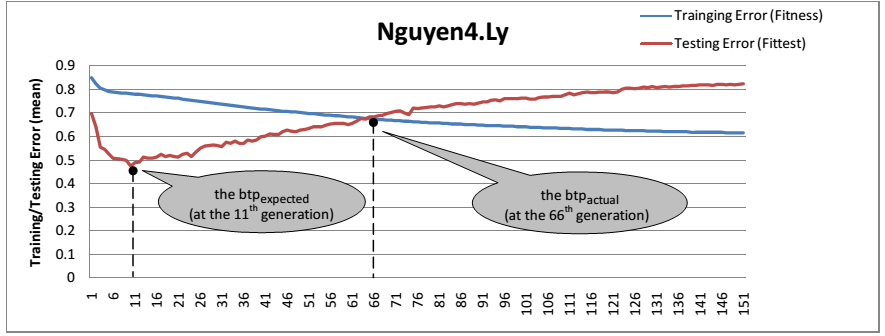
\includegraphics[scale=0.4]{Figures/Fig3_2.png}
% figure caption is below the figure
\caption{The case arises the second issue with the overfitting measurement proposed by Silva and colleagues.}
\label{fig:issue2.1}       % Give a unique label
\end{figure}

% For one-column wide figures use
\begin{figure}
% Use the relevant command to insert your figure file.
% For example, with the graphicx package use
\centering
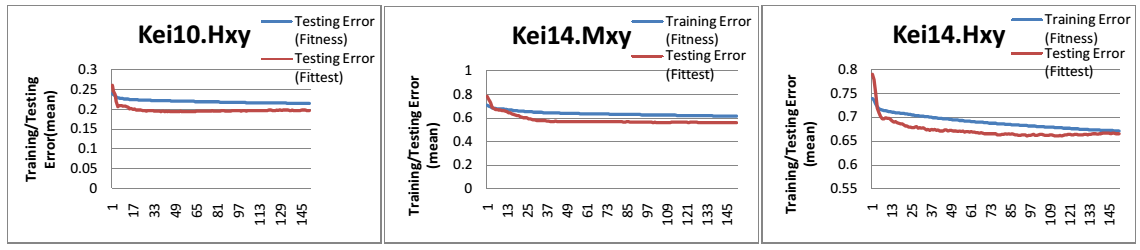
\includegraphics[scale=0.4]{Figures/Fig3_3.png}
% figure caption is below the figure
\caption{The more cases arise the second issue with the overfitting measurement proposed by Silva and colleagues.}
\label{fig:issue2.2}       % Give a unique label
\end{figure}


\subsubsection{Our proposed overfitting measurement}
In this section, we introduce a new method to quantify overfitting, to overcome the limits of the overfitting measurement proposed by Silva. This measurement is, in turn, used to classify our proposed benchmarks.

\begin{enumerate}
\item \textit{The new method to quantifying the OV at a generation g}\\
Using the same terminology by Silva et al., assuming that the best test point is at generation ${g}_{btp}$; $g$ is the current generation; $btp$ represents the best fitness error reached from when beginning of the run up until the current generation. As shown in Algorithm 1, the amount of over-fitting at generation $g$ is calculated as follows (for more details, see Figure \ref{fig:OV}):
\begin{eqnarray}
overfit(g)&=&{|training\_fit(g)-test\_fit(g)| - |tbtp-btp|} \nonumber\\
		  &=& {CF-AB}	\nonumber\\
          &=& {CF-DE}	\nonumber\\
		  &=& {|test\_fit(g) - btp|+|training\_fit(g)- tbtp|} \nonumber\\
		  &=& {CD+EF}  \nonumber\\
		  &=& {a_{g}+b_{g}}  \nonumber\\
\end{eqnarray}

% For one-column wide figures use
\begin{figure}
% Use the relevant command to insert your figure file.
% For example, with the graphicx package use
\centering
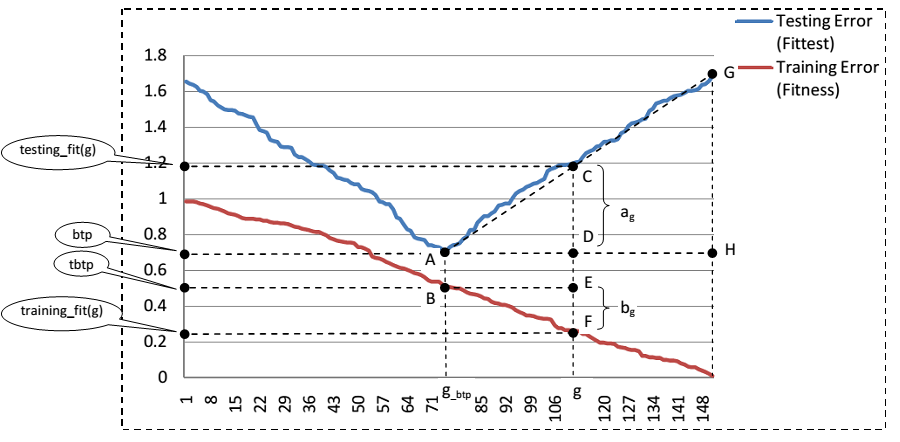
\includegraphics[scale=0.4]{Figures/Fig3_4.png}
% figure caption is below the figure
\caption{Graph for calculating the overfitting}
\label{fig:OV}       % Give a unique label
\end{figure}

It is noted that by using elitism mechanism in GP, $training\_fit(g)$ is always less than or equal to $tbtp$ at current generation $g$. Furthermore, in \cite{1996Mitchell}, the over-fitting be defined as follows:\textit{\textquotedblleft Given a hypothesis space $H$, a hypothesis $h \in H$ is said to overfit on the training sample if there exists some alternative hypothesis ${h}^{'} \in H$, such that $h$ has smaller error than ${h}^{'}$ over the training sample, but ${h}^{'}$ has smaller error than $h$ over the entire distribution of instances\textquotedblright}. This definition helps us not only find the best test point but also realize that the overfitting can be quantified independently to training error. So, in order to exactly reflect the amount of over-fitting at a generation, in the new overfitting formula we eliminate the quantity of $b_{g}$. Therefore, the new measure to quantify the amount of over-fitting at generation $g$ now is:
\begin{equation}
overfit (g) = a_{g} 	
\end{equation} \par

Besides, to overcome the issues that the Silva's method might face, We decide removing the condition (1) in this method. The details of our overfitting measure as shown in the algorithm 2 below.

\item \textit{The new method to quantify overfitting of problems} \\
We have mentioned the new overfitting measure at generation g. In order to quantify the overfitting of a problem, besides considering the amount of over-fitting  at the final generation, we should also pay attention to the early (or late) over-fitted characteristic of problem. Therefore, the overfitting of a problem should reflect two characteristics including the overfitting at the final generation and the generation that overfitting begins. This means: the more the over-fitting of a problem, the more the overfitting at the final generation and the earlier the beginning of over-fitting. To reflect these characteristics, we see the overfitting of a problem (OV) as the square root of the half area of the triangle AGH (see the Figure \ref{fig:OV}), or 
\begin{equation}
OV=\sqrt{(a_{n}*(n-{g}_{btp}))/2} 
\end{equation}
where, $n$ is the number of generations; $btp$ is the best test point found after running from generation $1$ to generation $n$;  $a_{n}$ is the mount of over-fitting at the final generation, $n$. Algorithm 2 presents the description of our new method. It is noted that by incorporating the starting time (generation) for overfitting into the calculation, our measurement is different from those proposed in \cite{2008Trevor}\cite{Marcel}\cite{copas1983regression}\cite{bilger2015measuring}, where the amount of overfitting is only calculated at the end of the training process. We believe this type of overfitting quantification is more suitable for learning machines with iterative training as GP.
\begin{table}
\begin{tabular}{lllllllllll}
\multicolumn{11}{l}{\textbf{Algorithm 2}: The new overfitting measurement} \\
\multicolumn{1}{l|}{} & \multicolumn{10}{l}{$overfit(0) = 0$} \\
\multicolumn{1}{l|}{} & \multicolumn{10}{l}{$btp = test\_fit(0)$} \\
\multicolumn{1}{l|}{} & \multicolumn{10}{l}{$tbtp = training\_fit(0)$} \\
\multicolumn{1}{l|}{} & \multicolumn{10}{l}{\textbf{for each } $generation$ $g>0$ } \\
\multicolumn{1}{l|}{} & \multicolumn{1}{l|}{} & \multicolumn{9}{l}{  \textbf{if} $(test\_fit(g) < btp)$} \\
\multicolumn{1}{l|}{} & \multicolumn{1}{l|}{} & \multicolumn{1}{l|}{} & \multicolumn{8}{l}{$overfit(g)= 0$} \\
\multicolumn{1}{l|}{} & \multicolumn{1}{l|}{} & \multicolumn{1}{l|}{} & \multicolumn{8}{l}{$btp = test\_fit(g)$} \\
\multicolumn{1}{l|}{} & \multicolumn{1}{l|}{} & \multicolumn{1}{l|}{} & \multicolumn{8}{l}{${g}_{btp}= g$} \\
\multicolumn{1}{l|}{} & \multicolumn{1}{l|}{} & \multicolumn{9}{l}{\textbf{else}} \\
\multicolumn{1}{l|}{} & \multicolumn{1}{l|}{} & \multicolumn{1}{l|}{} & \multicolumn{8}{l}{ $overfit(g) = |test\_fit(g) - btp| $} \\
\multicolumn{1}{l|}{} & \multicolumn{1}{l|}{} & \multicolumn{9}{l}{\textbf{endif}} \\
\multicolumn{1}{l|}{} & \multicolumn{10}{l}{\textbf{endfor}} \\
\multicolumn{1}{l|}{} & \multicolumn{10}{l}{$OV=\sqrt{overfit(n-1)*(n-{g}_{btp})/2}$ } \\
\multicolumn{1}{l|}{} & \multicolumn{10}{l}{\textbf{return} $OV$ } \\
\end{tabular}
\end{table}

\item \textit{Analyzing the effectiveness of the new overfitting measure}\\
By using our method (see Algorithm 2), the issue in Silva's measurement is solved. Considering problems shown in Figure \ref{fig:issue1} and Figure \ref{fig:issue2.2} (Kei10.Hxy, Kei11.My, Kei11.Hxy, Kei12.My, Kei14.Hy, Kei14.Mxy, Kei14.Hxy, Nguyen4.Mxy, Nguyen4.Ly), the corresponding best test points of these problems are precisely detected by this new method, occurring at the generation of 84, 0, 3, 6, 50, 106, 94, 27, 9, correspondingly. In addition, the corresponding overfitting values starting from generation ${g}_{btp}$ are also quantified.
\end{enumerate}
\end{enumerate}
%HOAI - is there any way to prove (in theorems) that the new measurement is better than Silva's one in that it does not have the issues rather than just give demonstrations on some data sets?

\subsection {Grouping the problems based on over-fitting (OV)}
\label{clus}
After using the new overfitting measure to quantify the overfitting of problems, we use the \textit{Gene Cluster 3.0} software, a k-means clustering algorithm, to clustering these problems based on their overfitting. \textit{Gene Cluster 3.0} is the open source cluster software created by Michael Eisen and Seiya (University of Tokyo, Human Genome Center June 2002) and available at link:\\
\textit{http://www.mediafire.com/file/pdjzff1r7e5hx7f/clustersetup.exe}.

\section{Experimental setting}
\label{Exp}
\subsection{Benchmark problems}
\label{Ben}
As shown in \cite{2015Mig} not all functions are suitable to be used as benchmarks. Here, we choose Symbolic Regression functions from \cite{2012James} as shown in Table \ref{tab:Problem}. There are two reasons for this selection: (1) These problems have not received much attention from Genetic Programming community \cite{David2013}; (2) they have various response variable distributions to ensure the best coverage. Figure ~\ref{fig:Distribute}) shows response variable distributions of these functions: Kei12, Val5, Vla6, Nguyen\_1 are quite like Normal Distribution; functions like Kei10, Kei11, Vla1 with a few outliers in one tailed; Kei 15, Vla5 with more evenly outlier in both 2-tailed; functions as Kei14, Vla8, Nguyen\_2, Nguyen\_3, Nguyen\_4 with much higher density of outliers and very skew making them very challenging. \par

Towards a synthesis for benchmark generation, and as shown in \cite{2015Mig}, all data sets generated from chosen functions have common features: the input range, how to sample the training and testing sets, the number of samples in the testing set are the same in \cite{2012James}. However, the size of the training set could be used to analyze the difficulty of the problem \cite{2015Mig}. Therefore, to control the difficulty of the problem by only the OV measurement, we generate training sets with 200 samples for all functions. This size is recommended by Thomas and Lee Spector in \cite{Thomas2015}. They recommended that for most problems, training cases should be between 100 and 200, depending on the difficulty of the problem as well as the dimensionality of the input space.
%\begin{landscape}
\begin{table}
% table caption is above the table
\caption{GP Benchmark Regression Problems}
\label{tab:Problem}       % Give a unique label
% For LaTeX tables use
\begin{tabular}{llll}
\hline\noalign{\smallskip}
Name &  Definition & Training Data  & Testing Data\\
\noalign{\smallskip}\hline\noalign{\smallskip}
Kei10 &	 $x_{1}^{x_{2}}$ & U[0, 1, 200]	& E[0, 1, 0.01] \\
Kei11 & $x_{1}x_{2}+\sin((x_{1}-10)(x_{2}-1))$& U[-3, 3, 200] & E[-3, 3, 0.01] \\
Kei12 & $x_{1}^4-x_{1}^3+\frac{x_{2}^2}{2}-x_{2}$ & U[-3, 3, 200]	& E[-3, 3, 0.01] \\
Kei13 & $\sin(x_{1})\cos(x_{2})$ & U[-3, 3, 200]	& E[-3, 3, 0.01] \\
Kei14 & $\frac{8}{2+x_{1}^2+x_{2}^2}$ & U[-3, 3, 200]	& E[-3, 3, 0.01] \\
Kei15 & $\frac{x_{1}^3}{5}+\frac{x_{2}^3}{2}-x_{2}-x_{1}$ & U[-3, 3, 200]	& E[-3, 3, 0.01] \\
Vla1 & $\frac{{e^{{(x_{1}-1)}^2}}}{1.2+(x_{2}-2.5)^2}$ & U[0.3, 4, 200] & E[-0.2, 4.2, 0.01] \\
Vla5 & $30\frac{(x_{1}-1)(x_{3}-1)}{x_{2}^2(x_{1}-10)}$ &
$\begin{array}{l} x_{1}: \textnormal{U}[0.05, 2, 200] \\ %U khong bi nghieng
x_{2}: \textnormal{U}[1, 2, 200]\\
x_{3}: \textnormal{U}[0.05, 2, 200] \end{array}$	& $\begin{array}{l} x_{1}: \textnormal{E}[-0.05, 2.1, 0.15]\\
x_{2}: \textnormal{E}[0.95, 2.05, 0.1] \\
x_{3}: \textnormal{E}[-0.05, 2.1, 0.15] \end{array} $\\
Vla6 & $6\sin(x_{1})\cos(x_{2})$ & U[0.1, 5.9, 200] & E[-0.05, 6.05, 0.02] \\
Val8 & $\frac{(x_{1}-3)^4+(x_{2}-3)^3-(x_{2}-3)}{(x_{2}-2)^4+10}$ & U[0.05, 6.05, 200] &	E[-0.25, 6.35, 0.2] \\
Nguyen\_1 & $ x^3+x^2+x $ & U[-1,1,200] & U[-1,1,100] \\
Nguyen\_2 & $ x^4+x^3+x^2+x $ & U[-1,1,200]	& U[-1,1,100] \\
Nguyen\_3 & $ x^5+x^4+x^3+x^2+x $ & U[-1,1,200]	& U[-1,1,100] \\
Nguyen\_4 & $ x^6+x^5+x^4+x^3+x^2+x $ & U[-1,1,200]	& U[-1,1,100] \\
\noalign{\smallskip}\hline
\end{tabular}
\end{table}
%\end{landscape}

% For one-column wide figures use
\begin{figure}
% Use the relevant command to insert your figure file.
% For example, with the graphicx package use
\centering
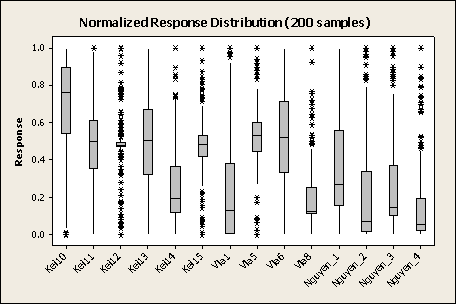
\includegraphics[scale=0.6]{Figures/Figure3.png}
% figure caption is below the figure
\caption{Normalized response variable distribution over 200 samples for each function (response variable normalized by the formula in \cite{2015Mig})}
\label{fig:Distribute}       % Give a unique label
\end{figure}


\subsection{GP Parameters Setting}
\label{GPP}
The GP parameters used for our experiments are shown in Table \ref{tab:Parameter}. These are typical settings often used by GP researchers and practitioners \cite{1992Koza}. To stabilize the variance of the intermediate quantities in the individual tree, we use an analytic quotient (AQ) operator \cite{Ni2013} instead of the protected division (PD).

\begin{table}
% table caption is above the table
\caption{Run and Evolutionary Parameters Values}
\label{tab:Parameter}       % Give a unique label
% For LaTeX tables use
\begin{tabular}{ll}
\hline\noalign{\smallskip}
Parameter & Value \\
\noalign{\smallskip}\hline\noalign{\smallskip}
Problems &	Shown in the Table \ref{tab:Problem}  \\
EA used in GP systems &	Elitist, generational, expression tree representation \\
Function set &	+, -, *, / (AQ) \\
Terminal set &	Regression variables and one random constant in [0.0, 1.0] \\
No. of generations	& 151 \\
Population size	& 500 \\
Tournament size &	4 \\
Tree creation	& Ramped half-and-half (depths of 2 to 6) \\
Max. tree depth	& 15 \\
Sub tree crossover rate	& 0.9 \\
Sub tree mutation rate & 0.1 \\
No.  of Runs & 51 \\
Fitness function & RMSE \\
\noalign{\smallskip}\hline
\end{tabular}
\end{table}

\section {Results and discussion}
\label{Res}

Our experimental results include the following criteria: the OV of the best learned model as shown in Table \ref{tab:OV}; the generalization error; the complexity of the best model. All criteria are averaged over 51 independent runs, as shown in Table \ref{tab:Fittest}, Table \ref{tab:size}.


\subsection {Grouping generated data sets by over-fitting (OV)}
\label{Gro}

Table \ref{tab:OV} presents 140 data sets which are grouped into four clusters based on their OVs. Each cluster includes benchmarks with increasing OVs. The clustering results are shown in Table \ref{tab:cluster} and Table \ref{tab:InfCluster}.  To achieve this, we use k-means clustering algorithm as mentioned in section \ref{clus}. We adopt Euclidean distance, repeat 100 times, and use the median rather than the mean centering because median is more robust against outliers. All datasets with detailed description can be downloaded from:\\ \textit{https://www.dropbox.com/s/udek9c9ww44cjbu/Data\%20sets.rar?dl=0}
%\begin{landscape}
\begin{table}
% table caption is above the table
\caption{Four groups of generated data sets were clustered by criteria OV}
\label{tab:cluster}       % Give a unique label
% For LaTeX tables use
%a) Four groups of data sets were clustered by criteria OV
\begin{tabular}{lllll}
%\multicolumn{6}{l}{a) Four groups of generated data sets were clustered by criteria OV} \\
\hline\noalign{\smallskip}
& \multicolumn{4}{c}{Name of data set (Index of data set)} \\
\noalign{\smallskip}\hline\noalign{\smallskip}
& Kei2.My & Kei12.Ly & Kei12.Hy & Kei12.Hxy \\
Cluster 0 & Kei12.Hx & Kei12.Mx & Nguyen\_4.Ly & Kei11.My \\
(C0) & Kei11.Ly & Nguyen\_4.Hy & Kei11.Lxy & Vla1.Hx \\
& Nguyen\_4.Hx & & & \\
\hline
& Vla1.Lxy & Nguyen\_4.My & Kei12.Lx & Vla8.My \\
& Vla1.Hy & Nguyen\_4.Lx & Kei10.Hy & Nguyen\_3.Mxy \\
& Vla5.Lxy & Kei13.Hy & Kei14.Mxy & Vla8.Hxy \\
& Vla8.Hy & Vla6.Mx & Kei14.Lx & Vla8.Mx \\
& Kei10.Mxy & Kei13.My & Vla1.Mx & Kei13.My \\
& Vla6.My & Nguyen\_4.Mx & Vla6.Hy & Kei13.Mxy \\
Cluster 1 & Nguyen\_2.Mx & Vla5.My & Nguyen\_2.Ly & Kei13.Ly \\
(C1) & Vla1.Lx & Vla1.Ly & Vla6.Ly & Kei15.Mx \\
& Vla8.Lx & Kei10.Mx & Kei10.Ly & Kei10.Ly \\
& Kei14.Lxy & Kei10.Lxy & Kei10.F & Kei11.F \\
& Kei12.F & Kei13.F & Kei14.F & Kei15.F \\
& Vla1.F & Vla5.F & Vla6.F & Vla8.F \\
& Nguyen\_1.tr10 & Nguyen\_2.F & Nguyen\_3.F & Nguyen\_4. F \\
& Kei13.Lx & Kei15.Lx & Vla6.Lx & Nguyen\_3.Ly \\
& Vla5.Ly & Vla8.Ly & Vla6.Lxy & Vla8.Lxy \\
& Nguyen\_1.Lxy & Vla6.Mxy & Nguyen\_1.Mxy & \\
\hline
& Nguyen\_1.My & Kei14.My & Vla5.Hy & Nguyen\_4.Lxy \\
& Kei15.Hx & Kei11.Mxy & Kei14.Hy & Kei14.Ly \\
& Nguyen\_2.Lx & Vla5.Hxy & Vla6.Hxy & Kei14.Hx \\
& Vla8.Hx & Kei14.Mx & Nguyen\_1.Hx & Vla1.My \\
Cluster 2 & Vla5.Mxy & Nguyen\_1.Mx & Nguyen\_2.Hxy & Nguyen\_3.Mx\\
(C2) & Kei10.Hxy & Nguyen\_1.Hxy & Kei14.Hxy & Vla6.Hx \\
& Kei15.Lxy & Kei13.Hx & Kei10.Hx & Vla5.Hx \\
& Vla1.Hxy & Kei15.Ly  & Nguyen\_2.Lxy & Vla5.Lx \\
& Kei10.My & Vla5.Mx & Vla1.Mxy & Kei13.Lxy \\
& Nguyen\_3.Lxy & Kei12.Lxy & & \\
\hline
& Kei11.Hy & Nguyen\_3.Hy & Nguyen\_4.Hxy & Nguyen\_4.Mxy \\
& Kei11.Mx & Nguyen\_2.Hy & Kei12.Mxy & Kei15.Hy \\
Cluster 3 & Kei11.Lx & Kei11.Hxy & Nguyen\_2.Mxy & Kei15.Mxy \\
(C3) & Nguyen\_2.My & Nguyen\_3.Ly & Nguyen\_3.Hx & Nguyen\_1.Ly \\
& Kei15.My & Nguyen\_3.My & Nguyen\_1.Lx & Nguyen\_1.Hy \\
& Vla8.Mxy & Kei13.Hxy & Nguyen\_2.Hx & Nguyen\_3.Hxy \\
& Kei15.Hxy & Kei11.Hx & & \\

\noalign{\smallskip}\hline
\end{tabular}
\end{table}
%b) clustering information \\
\begin{table}
% table caption is above the table
\caption{ Information of clusters}
\label{tab:InfCluster}       % Give a unique label
\begin{tabular}{lllll}
%\multicolumn{5}{l}{b) clustering information} \\
\hline\noalign{\smallskip}
& Cluster 0 & Cluster 1 & Cluster 2 & Cluster 3 \\
\noalign{\smallskip}\hline\noalign{\smallskip}
No. of observations	& 13 &	63 &	38 &	26 \\
Within cluster sum of squares &	592.7936 &	0.28177 &	1.447554	& 11.98758 \\
Average distance from centroid &	4.256253 &	 0.049527	& 0.146812 &	0.527065 \\
Max distance from centroid	& 15.390471 &	0.168109 &	0.453639 &	1.491932 \\
Cluster centroids &	4.949519	& 0.021502 &	0.386764 &	1.385605 \\
Distances between centroids  & $\begin{array}{l}  C0 \rightarrow C1:\\
4.928017 \\
C0 \rightarrow C2:\\
4.562755 \\
C0 \rightarrow C3:\\
3.563914 \end{array}$ & $\begin{array}{l} C1 \rightarrow C2:\\
0.365262 \\
C1 \rightarrow C3:\\
1.364103 \end{array}$ & $\begin{array}{l} C2 \rightarrow C3:\\
0.998841 \end{array}$ & \\
OV range: [min, max] & $\begin{array}{l}	[3.186061,\\
20.33999] \end{array}$ & $\begin{array}{l}	[0,\\
0.189611]\end{array}$ & $\begin{array}{l} [0.208218,\\
0.841303] \end{array}$ & $\begin{array}{l} [0.913296, \\ 2.877537] \end{array}$\\
OV level &	High &	Free &	Low	& Medium \\
\noalign{\smallskip}\hline
\end{tabular}
\end{table}
%\end{landscape}

%\begin{landscape}
\begin{center}
\begin{table}
% table caption is above the table
\caption{Mean of OVs of the best model trained on generated data sets using the formula (3)}
\label{tab:OV}       % Give a unique label
% For LaTeX tables use
\begin{tabular}{lllllllllll}
\hline\noalign{\smallskip}
& F & Lx & Mx & Hx & Ly & My & Hy & Lxy & Mxy & Hxy  \\
\noalign{\smallskip}\hline\noalign{\smallskip}
Kei10 & 0 & 0.01 & 0.01 & 0.30 & 0.01 & 0.26 & 0.14 & 0.00 & 0.09 & 0.37 \\
Kei11 & 0 & 1.89 & 2.44 & 0.91 & 4.40 & 4.82 & 2.88 & 3.99 & 0.71 & 1.82 \\
Kei12 & 0 & 0.18 & 4.96 & 9.31 & 18.70 & 20.34 & 15.10 & 0.21 & 2.03 & 11.13 \\
Kei13 & 0 & 0.00 & 0.09 & 0.31 & 0.04 & 0.09 & 0.13 & 0.24 & 0.06 & 1.04 \\
Kei14 & 0 & 0.10 & 0.43 & 0.51 & 0.65 & 0.82 & 0.68 & 0.01 & 0.12 & 0.36 \\
Kei15 & 0 & 0.00 & 0.02 & 0.71 & 0.28 & 1.21 & 1.96 & 0.33 & 1.74 & 1.00 \\
Vla1 & 0 & 0.04 & 0.09 & 3.70 & 0.04 & 0.43 & 0.16 & 0.19 & 0.24 & 0.30 \\
Vla5 & 0 & 0.26 & 0.25 & 0.30 & 0.00 & 0.05 & 0.81 & 0.13 & 0.41 & 0.59 \\
Vla6 & 0 & 0.00 & 0.10 & 0.34 & 0.04 & 0.08 & 0.06 & 0.00 & 0.00 & 0.52 \\
Vla8 & 0 & 0.01 & 0.10 & 0.44 & 0.00 & 0.17 & 0.11 & 0.00 & 1.10 & 0.11 \\
Nguyen\_1 & 0 & 1.12 & 0.40 & 0.43 & 1.28 & 0.84 & 1.10 & 0.00 & 0.00 & 0.37 \\
Nguyen\_2 & 0 & 0.65 & 0.05 & 1.03 & 0.05 & 1.40 & 2.29 & 0.28 & 1.75 & 0.39 \\
Nguyen\_3 & 0 & 0.00 & 0.38 & 1.30 & 1.37 & 1.15 & 2.79 & 0.21 & 0.14 & 1.02 \\
Nguyen\_4 & 0 & 0.15 & 0.08 & 3.19 & 4.95 & 0.19 & 4.12 & 0.78 & 2.63 & 2.72 \\


\noalign{\smallskip}\hline
\end{tabular}
\end{table}
\begin{table}
% table caption is above the table
\caption{Fittest (mean) of the best learned model by GP with noise configurations}
\label{tab:Fittest}       % Give a unique label
% For LaTeX tables use
\begin{tabular}{lllllllllll}
\hline\noalign{\smallskip}
Problem & F & Lx & Mx & Hx & Ly & My & Hy & Lxy & Mxy & Hxy  \\
\noalign{\smallskip}\hline\noalign{\smallskip}
Kei-10 & 0.05 & 0.08 & 0.12 & 0.17 & 0.07 & 0.10 & 0.16 & 0.07 & 0.16 & 0.20 \\
Kei-11 & 0.56 & 0.91 & 1.66 & 2.33 & 0.96 & 1.18 & 1.56 & 1.03 & 2.47 & 2.70 \\
Kei-12 & 1.83 & 24.0 & 31.2 & 45.8 & 18.8 & 39.2 & 40.4 & 14.7 & 45.2 & 56.0 \\
Kei-13 & 0.67 & 1.41 & 2.05 & 2.34 & 0.96 & 1.68 & 2.19 & 1.35 & 2.60 & 2.70 \\
Kei-14 & 0.10 & 0.22 & 0.32 & 0.59 & 0.19 & 0.27 & 0.42 & 0.35 & 0.56 & 0.67 \\
Kei-15 & 0.73 & 0.97 & 1.68 & 2.44 & 1.43 & 1.46 & 2.55 & 1.39 & 2.56 & 3.19 \\
Vla-1 & 0.07 & 0.07 & 0.10 & 1.86 & 0.09 & 0.11 & 0.12 & 0.08 & 0.13 & 0.19 \\
Vla-5 & 0.34 & 0.44 & 0.66 & 0.62 & 0.36 & 0.47 & 0.65 & 0.53 & 0.75 & 0.74 \\
Vla-6 & 1.99 & 2.10 & 2.54 & 2.66 & 2.09 & 2.22 & 2.39 & 2.19 & 2.45 & 2.80 \\
Vla-8 & 1.12 & 1.59 & 1.89 & 2.17 & 1.33 & 1.51 & 2.13 & 1.61 & 2.10 & 2.26 \\
Nguyen-1 & 0.00 & 0.12 & 0.28 & 0.32 & 0.13 & 0.30 & 0.49 & 0.12 & 0.45 & 0.61 \\
Nguyen-2 & 0.01 & 0.06 & 0.17 & 0.47 & 0.11 & 0.29 & 0.72 & 0.17 & 0.42 & 0.50 \\
Nguyen-3 & 0.01 & 0.05 & 0.29 & 0.47 & 0.13 & 0.44 & 0.80 & 0.24 & 0.64 & 0.68 \\
Nguyen-4 & 0.02 & 0.14 & 0.65 & 0.93 & 0.82 & 0.58 & 1.09 & 0.54 & 0.71 & 1.49 \\
Mean & 0.53 & 2.30 & 3.11 & 4.51 & 1.96 & 3.56 & 3.97 & 1.74 & 4.37 & 5.34 \\

\noalign{\smallskip}\hline
\end{tabular}
\end{table}

\begin{table}
% table caption is above the table
\caption{Model complexity (mean) of the best learned model by GP with noise configurations}
\label{tab:size}       % Give a unique label
% For LaTeX tables use
\begin{tabular}{lllllllllll}
\hline\noalign{\smallskip}
Problem & F & Lx & Mx & Hx & Ly & My & Hy & Lxy & Mxy & Hxy  \\
\noalign{\smallskip}\hline\noalign{\smallskip}
Kei-10 & 270 & 311 & 338 & 348 & 288 & 315	& 338 &	331	& 309 & 288 \\
Kei-11 & 348 & 349 & 360 & 387 & 399 & 352 & 377 & 364 & 405 & 420 \\
Kei-12 & 291 & 408 & 473 & 442 & 381 & 414 & 428 & 376 & 447 & 531 \\
Kei-13 & 355 & 377 & 440 & 422 & 378 & 383 & 401 & 356 & 447 & 420 \\
Kei-14 & 205 & 261 & 276 & 284 & 259 & 257 & 270 & 258 & 262 & 271 \\
Kei-15 & 311 & 338 & 328 & 394 & 346 & 355 & 389 & 332 & 391 & 396 \\
Vla-1 & 328 & 312 & 341 & 324 & 339 & 337 & 359 & 329 & 324 & 342 \\
Vla-5 & 278 & 361 & 362 & 400 & 324 & 346 & 380 & 357 & 442 & 425 \\
Vla-6 & 399 & 410 & 410 & 389 & 391 & 414 & 428 & 415 & 415 & 407 \\
Vla-8 & 381 & 391 & 358 & 338 & 373 & 372 & 334 & 371 & 337 & 315 \\
Nguyen-1 & 159 & 331 & 406 & 402 & 354 & 380 & 380 & 396 & 411 & 453 \\
Nguyen-2 & 220 & 331 & 481 & 420 & 351 & 385 & 476 & 405 & 410 & 408 \\
Nguyen-3 & 245 & 288 & 382 & 406 & 381 & 405 & 390 & 365 & 423 & 435 \\
Nguyen-4 & 254 & 304 & 423 & 442 & 472 & 404 & 425 & 432 & 432 & 482 \\
Kei-10 & 426 & 411 & 420 & 449 & 405 & 427 & 361 & 403 & 411 & 476 \\
\noalign{\smallskip}\hline
\end{tabular}
\end{table}
\end{center}
%\end{landscape}

\subsection {Analysis of the robustness of GP to noise}
\label{AnaFittest}

Experimental results show that for all three noise types (noise x, noise y, noise x \& y), in most benchmark functions of interest, the greater the magnitude of noise, the greater the test error of the best solution (cases shown in bold in Table \ref{tab:Fittest}). Figure \ref{fig:Fittest} shows this more obviously. A reason for this could be due to the increasing level of noise which makes our benchmarks more difficult to learn the exact models. The training (fitness) errors in some functions are shown in Figure ~\ref{fig:Fitness} (graph of all functions can be download from https://www.dropbox.com/s/gnuinkzicoq9jdr/Graph.rar?dl=0). 
It can be seen that the fitness error of the best model with noise level 0\% is smaller than that with 10\% noise ($finess(0 \%) < fitness(10\%)$); similarly, $finess(10\%) < fitness(30\%)$; $fitness(30\%) < fitness(50\%)$. \par

It can also be observed that increasing noise magnitude reduces the generalization ability, and also increases the complexity of learned models in most cases ( Table \ref{tab:size}). Thus, it is reasonable to conclude that GP is not a robust-to-noise Machine Learning technique, at least for the problem of interest in this paper.
\begin{figure}
% Use the relevant command to insert your figure file.
% For example, with the graphicx package use
  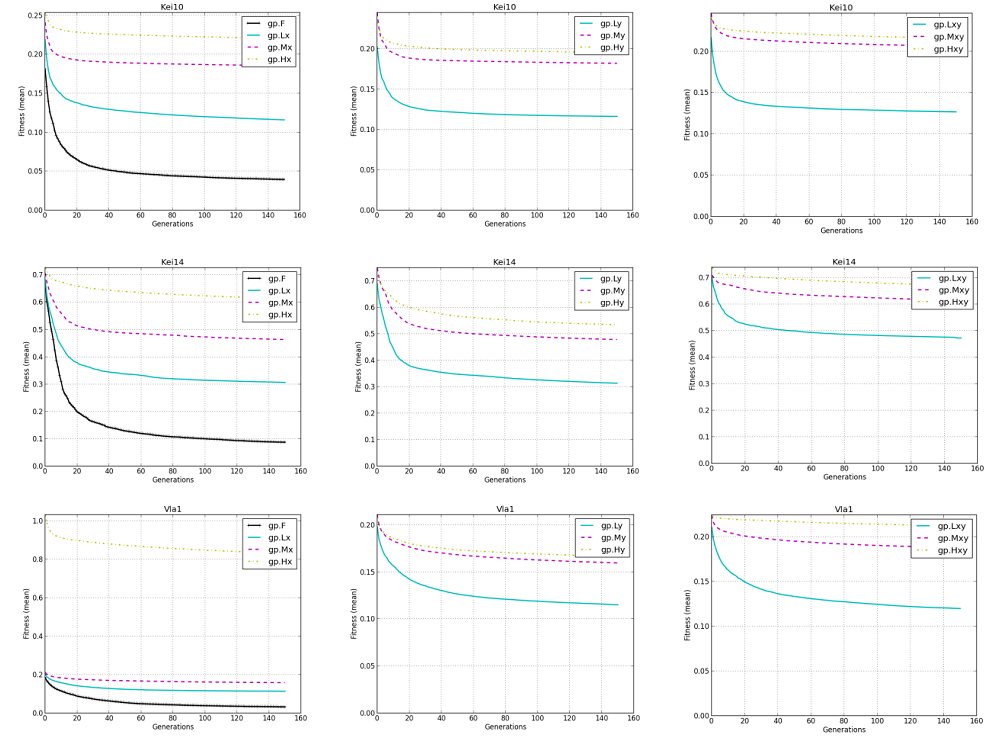
\includegraphics[width=1.0\textwidth]{Figures/Figure4.png}
  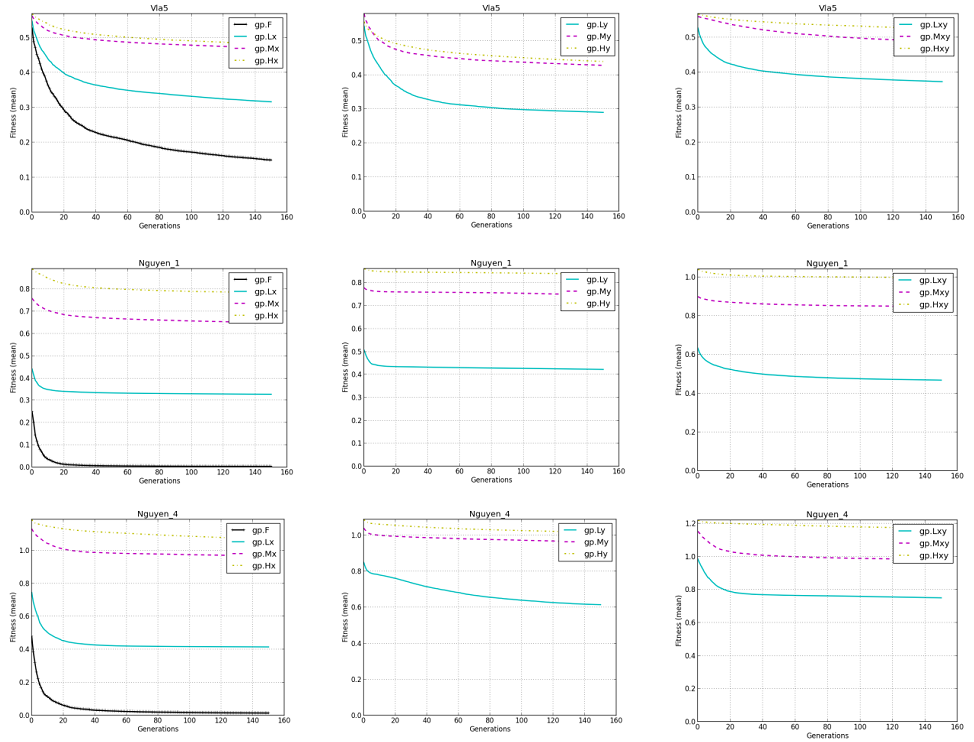
\includegraphics[width=1.0\textwidth]{Figures/Figure5.png}
 % figure caption is below the figure
\caption{Fitness (mean) of the best learned model by GP with noise configurations}
\label{fig:Fitness}       % Give a unique label
\end{figure}
\begin{figure}
% Use the relevant command to insert your figure file.
% For example, with the graphicx package use
  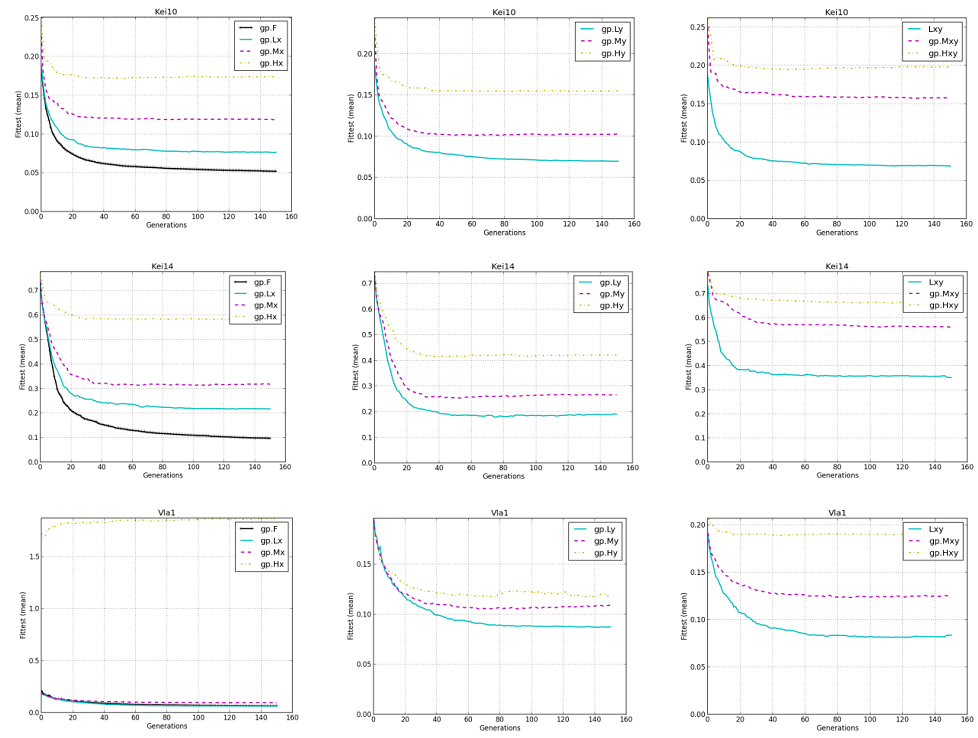
\includegraphics[width=1.0\textwidth]{Figures/Figure7.png}
  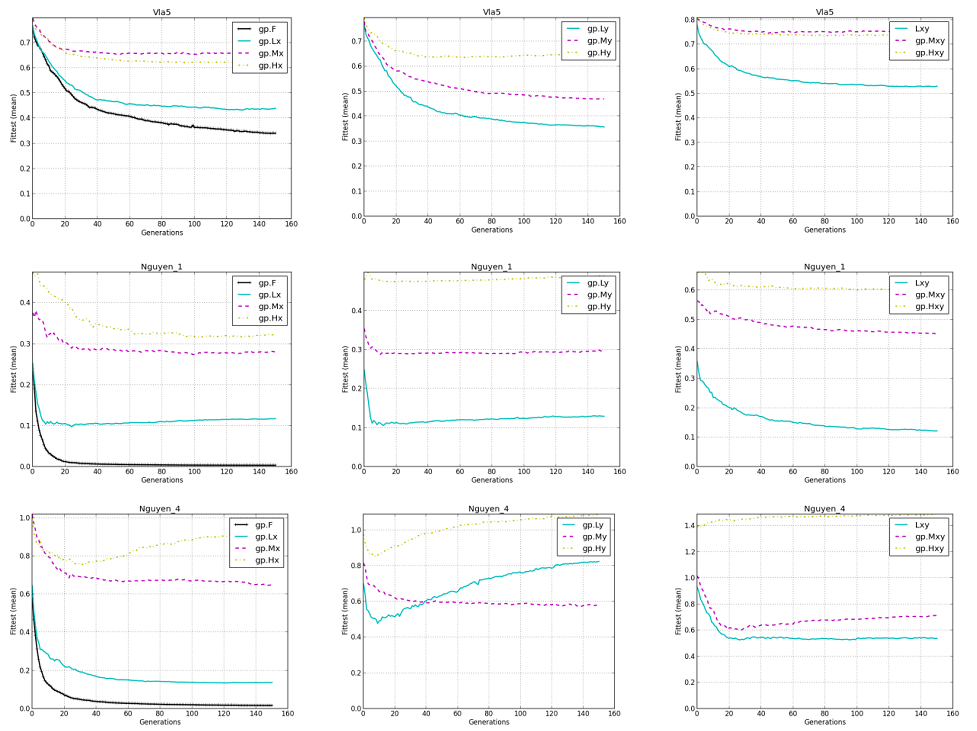
\includegraphics[width=1.0\textwidth]{Figures/Figure8.png}
 % figure caption is below the figure
\caption{Fittest (mean) of the best learned model by GP with noise configurations}
\label{fig:Fittest}       % Give a unique label
\end{figure}


\subsection {Noise types and noise levels analysis}
\label{AnaDiff}
Beside some common features shown in section \ref{AnaFittest}, each noise type and magnitude shows a few distinctive characteristics: (1) the volume of test error; (2) the convergence rate; (3) the generalization ability of the solution. To show how different each noise setting is, we use a function: sign(x): returns (+) if $x>0$ else returns (-).


\subsubsection{Test error analysis}
\label{AnaDiffMag}

For most of the problems with the same noise level and the same function, the test error of model solutions that are trained on data set with noise x,y is often less than that are trained on data set with noise xy.

\begin{itemize}
\item Consider the case between noise x and noise xy: in most benchmark functions, the test error of the best model on original data with noise x is often less than that with noise xy. In Table \ref{tab:difFittest}, negative (-) cases show the test error with noise xy is less than with noise x. It is true on 11 over 14 functions (including Kei11, Kei14, Kei15, Vla1, Vla5, Vla6, Vla8, Nguyen\_1, Nguyen\_2, Nguyen\_3 and Nguyen-4) with noise level at 10\%; and on 13 over 14 problems with noise level 30\%, and 50\% as well.

\item Consider the case between noise y and noise xy: there are 8/14, 14/14, 12/14 functions at the noise level of 10\%, 30\%, 12\%, respectively, in which the test errors with noise y are less than with noise xy.

\item Consider the case between noise x and noise y: The difference now is not clear. The number of problems with noise x having better test errors than with noise y are 7/14; 5/14; 6/14, with noise level 10\%, 30\%, 50\%, respectively.

\end{itemize} \par
%\begin{landscape}
\begin{table}
\caption{The difference in the test error of the best models with various noise types: (a) sign(Fittest(Noise x) - Fittest(Noise y)); (b) sign(Fittest(Noise x) - Fittest(Noise xy)); c) sign(Fittest(noise y)-Fittest(noise xy)}
\label{tab:difFittest}       % Give a unique label
\begin{tabular}{l|lll|lll|lll}
\hline\noalign{\smallskip}
Problem & \multicolumn{3}{c|}{(a)} & \multicolumn{3}{c|}{(b)} & \multicolumn{3}{c}{(c)} \\
 & \multicolumn{1}{c}{\textit{10\%}} & \multicolumn{1}{c}{\textit{30\%}} & \multicolumn{1}{c|}{\textit{50\%}} & \multicolumn{1}{c}{\textit{10\%}} & \multicolumn{1}{c}{\textit{30\%}} & \multicolumn{1}{c|}{\textit{50\%}} & \multicolumn{1}{c}{\textit{10\%}} & \multicolumn{1}{c}{\textit{30\%}} & \multicolumn{1}{c}{\textit{50\%}} \\
\hline
Kei10 & + & + & + & + & - & - & + & - & - \\
Kei11 & - & + & + & - & - & - & - & - & - \\
Kei12 & + & - & + & + & - & - & + & - & - \\
Kei13 & + & + & + & + & - & - & - & - & - \\
Kei14 & + & + & + & - & - & - & - & - & - \\
Kei15 & - & + & - & - & - & - & + & - & - \\
Vla1 & - & - & + & - & - & + & + & - & - \\
Vla5 & + & + & - & - & - & - & - & - & - \\
Vla6 & + & + & + & - & + & - & - & - & - \\
Vla8 & + & + & + & - & - & - & - & - & - \\
Nguyen\_1 & - & - & - & - & - & - & + & - & - \\
Nguyen\_2 & - & - & - & - & - & - & - & - & + \\
Nguyen\_3 & - & - & - & - & - & - & - & - & + \\
Nguyen\_4 & - & + & - & - & - & - & + & - & - \\
\hline
\end{tabular}
\end{table}


\subsubsection {Convergence rate analysis}
\label{AnaDiffCR}

To show how noise relates to the convergence rate of the solution, we calculate the mean of convergence rate over generations by taking fitness error of previous generation minus the same error of later generation, repeating through a cumulative process, then getting the average.

Results in the Table \ref{tab:CR} shows that: (1) With the same noise type, the convergence rate is decreased when the magnitude of noise is increased in most benchmark functions. Table \ref{tab:difCR1} is built from Table \ref{tab:CR} in which cells with sign (+) indicate $CR(0\% noise) > CR(10\% noise)$ ;$ CR(10\%) > CR(30\%)$ and $ CR(30\%) > CR(50\%)$. It can be seen in Table \ref{tab:difCR1} that the observation is true for all noise types; (2) in Table \ref{tab:difCR2}, most of our functions, with the same level of noise, the convergence rate of the best model on the data set with noise x, y is bigger than on the data set with noise xy, especially when noise is increased. However, this distinction is not clear between noise x and noise y:
\begin{enumerate}
\item Considering the case of noise x and noise xy:
\begin{enumerate}
\item At the level of noise by 10\%, there are 9 functions from 14 benchmark functions: Kei10, Kei11, Kei14, Kei15, Vla1, Vla5, Vla6 Nguyen-3, Nguyen-4 have $CR(noise x) > CR(noise xy)$.
\item At the level of noise by 30\%, all benchmark  functions  (except Kei11, Vla6, Nguyen-4) have $CR(noise x) > CR(noise xy)$ (11/14 functions).
\item At the level of noise by 50\%, all benchmark  functions have $ CR(noise x) > CR(noise xy)$ (14/14 functions).
\end{enumerate}
\item Considering the case of noise y and noise xy: At the levels of noise by 10\%, 30\%, 50\%, respectively, there are 8/14, 10/14, 13/14 functions which the convergence rate of the best learned model on data set with noise y is greater than on data set with noise xy.
\item Considering the case of noise x and noise y, the difference is not clear. At the levels of noise by 10\%, 30\%, 50\%, respectively, there are 8/14, 7/14, 7/14 functions in which the convergence rate of the best model on data set with noise x is greater than on data set with noise y.
\end{enumerate} \par

\begin{table}
% table caption is above the table
\caption{Mean of the convergence rate across generations (measured through the fitness error of the best model)}
\label{tab:CR}       % Give a unique label
% For LaTeX tables use
\begin{tabular}{lllllllllll}
\hline\noalign{\smallskip}
Problem & F & Lx & Mx & Hx & Ly & My & Hy & Lxy & Mxy & Hxy  \\
\noalign{\smallskip}\hline\noalign{\smallskip}
Kei10 & 9.E-04 & 7.E-04 & 4.E-04 & 2.E-04 & 6.E-04 & 4.E-04 & 3.E-04 & 6.E-04 & 3.E-04 & 2.E-04 \\
Kei11 & 1.E-03 & 4.E-03 & 2.E-03 & 2.E-03 & 2.E-03 & 2.E-03 & 2.E-03 & 2.E-03 & 2.E-03 & 1.E-03 \\
Kei12 & 3.E-01 & 2.E-01 & 1.E-01 & 7.E-02 & 2.E-01 & 8.E-02 & 6.E-02 & 2.E-01 & 6.E-02 & 4.E-02 \\
Kei13 & 1.E-02 & 6.E-03 & 3.E-03 & 2.E-03 & 9.E-03 & 5.E-03 & 2.E-03 & 7.E-03 & 2.E-03 & 2.E-03 \\
Kei14 & 4.E-03 & 3.E-03 & 2.E-03 & 8.E-04 & 3.E-03 & 2.E-03 & 1.E-03 & 2.E-03 & 7.E-04 & 5.E-04 \\
Kei15 & 9.E-03 & 8.E-03 & 3.E-03 & 2.E-03 & 6.E-03 & 4.E-03 & 3.E-03 & 5.E-03 & 2.E-03 & 2.E-03 \\
Vla1 & 1.E-03 & 6.E-04 & 4.E-04 & 1.E-03 & 6.E-04 & 4.E-04 & 3.E-04 & 6.E-04 & 3.E-04 & 9.E-05 \\
Vla5 & 3.E-03 & 2.E-03 & 6.E-04 & 6.E-04 & 2.E-03 & 1.E-03 & 8.E-04 & 1.E-03 & 5.E-04 & 3.E-04 \\
Vla6 & 8.E-03 & 5.E-03 & 2.E-03 & 2.E-03 & 5.E-03 & 4.E-03 & 3.E-03 & 4.E-03 & 2.E-03 & 1.E-03 \\
Vla8 & 6.E-03 & 3.E-03 & 2.E-03 & 1.E-03 & 4.E-03 & 3.E-03 & 1.E-03 & 4.E-03 & 1.E-03 & 4.E-04 \\
Nguyen\_1 & 2.E-03 & 8.E-04 & 7.E-04 & 7.E-04 & 6.E-04 & 2.E-04 & 2.E-04 & 1.E-03 & 4.E-04 & 3.E-04 \\
Nguyen\_2 & 2.E-03 & 1.E-03 & 2.E-03 & 4.E-04 & 8.E-04 & 4.E-04 & 2.E-04 & 1.E-03 & 8.E-04 & 4.E-04 \\
Nguyen\_3 & 3.E-03 & 2.E-03 & 1.E-03 & 1.E-03 & 1.E-03 & 7.E-04 & 7.E-04 & 2.E-03 & 6.E-04 & 5.E-04 \\
Nguyen\_4 & 3.E-03 & 2.E-03 & 1.E-03 & 8.E-04 & 2.E-03 & 5.E-04 & 5.E-04 & 2.E-03 & 1.E-03 & 3.E-04 \\
\noalign{\smallskip}\hline
\end{tabular}
\end{table}
%\end{landscape}


\begin{table}
% table caption is above the table
\caption{The difference in the convergence rate (CR) of the best model on the data sets having the same type of noise but various noise levels: (a) sign(CR(0\%)- CR(10\%)); (b) sign(CR(10\%)- CR(30\%)); (c) sign(CR(30\%)- CR(50\%)) }
\label{tab:difCR1}       % Give a unique label
% For LaTeX tables use
\begin{tabular}{l|lll|lll|lll}
\hline\noalign{\smallskip}
Problem & \multicolumn{3}{c|}{Noise x} & \multicolumn{3}{c|}{Noise y} & \multicolumn{3}{c}{Noise xy} \\
 & (a) & (b) & (c) & (a) & (b) & (c) & (a) & (b) & (c) \\
\noalign{\smallskip}\hline\noalign{\smallskip}
Kei10 & + & + & + & + & + & + & + & + & + \\
Kei11 & - & + & - & - & - & - & - & - & + \\
Kei12 & + & + & + & + & + & + & + & + & + \\
Kei13 & + & + & + & + & + & + & + & + & + \\
Kei14 & + & + & + & + & + & + & + & + & + \\
Kei15 & + & + & + & + & + & + & + & + & - \\
Vla1 & + & + & - & + & + & + & + & + & + \\
Vla5 & + & + & + & + & + & + & + & + & + \\
Vla6 & + & + & + & + & + & + & + & + & + \\
Vla8 & + & + & + & + & + & + & + & + & + \\
Nguyen\_1 & + & + & + & + & + & + & + & + & + \\
Nguyen\_2 & + & - & + & + & + & + & + & + & + \\
Nguyen\_3 & + & + & - & + & + & + & + & + & + \\
Nguyen\_4 & + & + & + & + & + & + & + & + & + \\
\noalign{\smallskip}\hline
\end{tabular}
\end{table}


\begin{table}
\caption{The difference in the convergence rate (CR) of the best model on the data sets have the same noise level but various noise types: (a) sign(CR (noise x) - CR (noise y)); (b) sign(CR (noise x) - CR (noise xy)); (c) sign(CR (noise y) - CR (noise xy))}
\label{tab:difCR2}
\begin{tabular}{l|lll|lll|lll}
\hline\noalign{\smallskip}
Problem & \multicolumn{3}{c|}{(a)} & \multicolumn{3}{c|}{(b)} & \multicolumn{3}{c}{(c)} \\
 & 10\% & 30\%  & 50\%  & 10\% & 30\% & 50\% & 10\% & 30\%  & 50\% \\
\noalign{\smallskip}\hline\noalign{\smallskip}
Kei10 & + & - & - & + & + & + & - & + & + \\
Kei11 & + & + & + & + & - & + & + & - & + \\
Kei12 & - & + & + & - & + & + & + & + & + \\
Kei13 & - & - & - & - & + & + & + & + & + \\
Kei14 & - & - & - & + & + & + & + & + & + \\
Kei15 & + & - & - & + & + & + & + & + & + \\
Vla1 & + & + & + & + & + & + & - & + & + \\
Vla5 & - & - & - & + & + & + & + & + & + \\
Vla6 & - & - & - & + & - & + & + & + & + \\
Vla8 & - & - & - & - & + & + & + & + & + \\
Nguyen\_1 & + & + & + & - & + & + & - & - & - \\
Nguyen\_2 & + & + & + & - & + & + & - & - & - \\
Nguyen\_3 & + & + & + & + & + & + & - & + & + \\
Nguyen\_4 & + & + & + & + & - & + & - & - & + \\
\noalign{\smallskip}\hline
\end{tabular}
\end{table}


\subsubsection {The difference in overfitting amount}
\label{AnaDiffOV}

Overfitting issue may be caused by training learning models on limited samples (eg, BEN-7-8 BEN, BEN-9 where the range of variables on the training set is smaller than on the testing set) or on samples containing noise. Results in Table \ref{tab:OV}, Table \ref{tab:difOV1}, and \ref{tab:difOV2} are used to analyze the impact of noise types and noise levels to the OV. \par

Noise types and noise levels have some common features: (1) The greater the noise level, the greater the OV. It is true with most benchmark functions (see cells(+) in the Table \ref{tab:difOV1}). For example, considering noise x, there are 14/14, 10/14, 13/14 functions that $OV (10\% noise) \ge OV (0\% noise)$; $OV(30\%) > OV(10\%)$ ; $OV(50\%) > OV(30\%)$. (2) with noise level by 50, all functions are over-fitted. Besides the above common features, they also have different characteristics, especially at noise level 30\%, OV (with noise y) is greater than OV with noise x and with noise xy) in most cases (see cells (-) in \ref{tab:difOV2}). This shows that noise y usually creates more over-fitting challenges than other types of noise.\par

\begin{table}
% table caption is above the table
\caption{The difference in OV of the best model trained on data sets with the same noise type but different noise levels: (a) sign(OV(10\% noise)-OV(0\% noise)); (b) sign(OV(30\% noise)-OV(10\% noise)); (c) sign(OV(50\% noise)-OV(30\% noise)) }
\label{tab:difOV1}       % Give a unique label
% For LaTeX tables use
\begin{tabular}{l|lll|lll|lll}
\hline\noalign{\smallskip}
Problem &\multicolumn{3}{|c|}{Noise x} & \multicolumn{3}{c|}{Noise y} & \multicolumn{3}{c}{Noise xy} \\
(a) & (b) & (c) & (a) & (b) & (c) & (a) & (b) & (c)\\
\noalign{\smallskip}\hline\noalign{\smallskip}
Kei10 & + & + & + & + & + & - & + & + & + \\
Kei11 & + & + & - & + & + & - & + & - & + \\
Kei12 & + & + & + & + & + & - & + & + & + \\
Kei13 & + & + & + & + & + & + & + & - & + \\
Kei14 & + & + & + & + & + & - & + & + & + \\
Kei15 & + & + & + & + & + & + & + & + & - \\
Vla1 & + & + & + & + & + & - & + & + & + \\
Vla5 & + & - & + & + & + & + & + & + & + \\
Vla6 & + & + & + & + & + & - & + & + & + \\
Vla8 & + & + & + & + & + & - & + & + & - \\
Nguyen\_1 & + & - & + & + & - & + & + & + & + \\
Nguyen\_2 & + & - & + & + & + & + & + & + & - \\
Nguyen\_3 & + & + & + & + & - & + & + & - & + \\
Nguyen\_4 & + & - & + & + & - & + & + & + & + \\
\noalign{\smallskip}\hline
\end{tabular}
\end{table}


\begin{table}
\caption{The difference in OV of the best model trained on data sets with the same noise level but different noise types: (a) sign(OV (noise x) - OV (noise y)); (b) sign(OV (noise x) - OV (noise xy)); (c) sign(OV (noise y) - OV (noise xy))}
\label{tab:difOV2}
\begin{tabular}{l|lll|lll|lll}
\hline\noalign{\smallskip}
Problem & \multicolumn{3}{c|}{(a)} & \multicolumn{3}{c|}{(b)} & \multicolumn{3}{c}{(c)} \\
 & 10\% & 30\% & 50\% & 10\% & 30\% & 50\% & 10\% & 30\% & 50\% \\
\noalign{\smallskip}\hline\noalign{\smallskip}
Kei10 & + & - & + & + & - & - & - & - & + \\
Kei11 & - & - & - & - & + & - & - & - & - \\
Kei12 & - & - & - & - & + & - & - & - & - \\
Kei13 & - & + & + & - & + & - & + & - & + \\
Kei14 & - & - & - & + & + & + & - & - & - \\
Kei15 & - & - & - & - & - & - & + & + & - \\
Vla1 & + & - & + & - & - & + & + & - & + \\
Vla5 & + & + & - & + & - & - & + & + & - \\
Vla6 & - & + & + & + & + & - & - & - & + \\
Vla8 & + & - & + & + & - & + & + & + & + \\
Nguyen\_1 & - & - & - & + & + & + & - & - & - \\
Nguyen\_2 & + & - & - & + & - & + & + & + & - \\
Nguyen\_3 & - & - & - & - & + & + & - & - & - \\
Nguyen\_4 & - & - & - & - & - & + & - & + & - \\


\noalign{\smallskip}\hline
\end{tabular}
\end{table}
%\end{landscape}


\section {Conclusions and future works}
\label{Con}
In this paper we have set out to understand the impact that noise might have on the generalization ability of a learning model. We also have proposed a method to quantify the over-fitting of benchmarks in GP, as well as developed a set of symbolic regression benchmarks which includes four groups with increasing (OV) difficulty levels. Different types of noise with different magnitudes are studied empirically to show whether GP is robust to noise or not. In summary, what has been achieved includes:

\begin{itemize}
\item A new measure to quantify the OV using the formula (3). It is a combination of two factors: the amount of over-fitting using the formula (2); over-fitting happens sooner or later when evolution best model over generations.

\item A set of benchmarks to study how robust a learning model is with the presence of noise. These data sets are grouped to four clusters based on their OVs. The volume of OV in Cluster 0, Cluster 3, Cluster 2 and Cluster 1 are assigned to \textquotedblleft high\textquotedblright, \textquotedblleft medium\textquotedblright, \textquotedblleft low\textquotedblright and \textquotedblleft free\textquotedblright by us. Data sets in each cluster are sorted in order of descending OV.

\item An analysis of the robustness of the GP to noise. Experimental results have shown that GP is very sensitive to noise. The higher the noise level, the lower the generalization ability of a GP learning model. This is the general feature which happens with all noise types and noise levels. However, each type of noise and each level of noise have its own characteristics that impact on the evolution of GP solutions, as analyzed in the section \ref{AnaDiff}. These characteristics include: (1) the magnitude of test error, 2) the convergence rate and 3) the OV of the best leaned model by GP. 

Moreover, in most problems, noise xy usually has (1) greater than noise x, y while (2) is lower. It can be seen that the higher the noise level, the greater the OV. So to study the generalization ability and over-fitting level of solutions training on a data set containing noise, we cannot just concern one noise type. To study the affect of noise on the test error and the convergence rate of a solution, we need to study a couple of noise types as $(noise xy; noise x)$ or $(noise y; noise xy)$. These are also our recommendations for researchers who aspire to  design benchmarks for these study goals.
\end{itemize} \par

There are several ways to further the findings in this work. First, future work will propose a more general method to quantify the OV for other iterative training based Machine Learning methods.  Second, it is necessary to conduct more experiments with other noise models to have more information about them. Last, we will conduct extensive experiments using different improved versions of GP on the benchmark proposed in this paper so as to investigate how these improvements would help GP to cope with increasing difficulties of learning to generalize.

%This distribution is built by bootstrap re-sampling method \cite{RefJ}.


%\label{sec:2}
%as required. Don't forget to give each section
%and subsection a unique label (see Sect.~\ref{sec:1}).
%\paragraph{Paragraph headings} Use paragraph headings as needed.

% For one-column wide figures use
%\begin{figure}
% Use the relevant command to insert your figure file.
% For example, with the graphicx package use
%  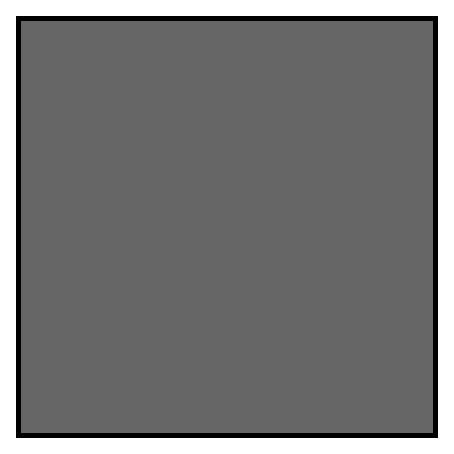
\includegraphics{example.eps}
% figure caption is below the figure
%\caption{Please write your figure caption here}
%\label{fig:1}       % Give a unique label
%\end{figure}
%
% For two-column wide figures use
%\begin{figure*}
% Use the relevant command to insert your figure file.
% For example, with the graphicx package use
 % 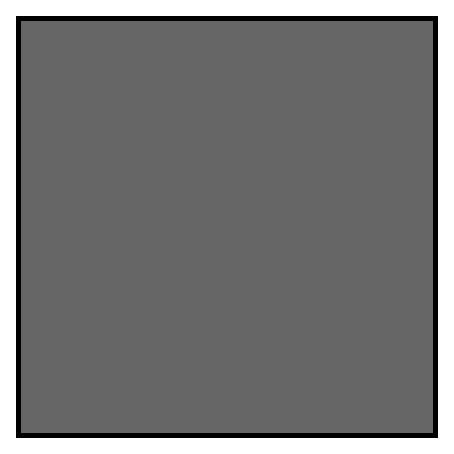
\includegraphics[width=0.75\textwidth]{example.eps}
% figure caption is below the figure
%\caption{Please write your figure caption here}
%\label{fig:2}       % Give a unique label
%\end{figure*}
%


\begin{acknowledgements}
%If you'd like to thank anyone, place your comments here
%and remove the percent signs.

\end{acknowledgements}

% BibTeX users please use one of
%\bibliographystyle{spbasic}      % basic style,
\bibliographystyle{plain}      % basic style,
% author-year citations

%\bibliographystyle{spmpsci}      % mathematics and physical sciences
%\bibliographystyle{spphys}       % APS-like style for physics
\bibliography{BibPaper2}   % name your BibTeX data base
%\printbibliography
% Non-BibTeX users please use
%\begin{thebibliography}{1}

%\bibliographystyle{IEEEtran}
%\bibliography{BibPaper2.bib}


% and use \bibitem to create references. Consult the Instructions
% for authors for reference list style.
%
%\bibitem{pa1}
% Format for Journal Reference
%Author, Article title, Journal, Volume, page numbers (year)
% Format for books
%\bibitem{RefB}
%Author, Book title, page numbers. Publisher, place (year)
% etc
%\end{thebibliography}

\end{document}
% end of file template.tex


%%%%%%%%%%%%%%%%%%%%%%% file template.tex %%%%%%%%%%%%%%%%%%%%%%%%%
%
% This is a general template file for the LaTeX package SVJour3
% for Springer journals.          Springer Heidelberg 2010/09/16
%
% Copy it to a new file with a new name and use it as the basis
% for your article. Delete % signs as needed.
%
% This template includes a few options for different layouts and
% content for various journals. Please consult a previous issue of
% your journal as needed.
%
%%%%%%%%%%%%%%%%%%%%%%%%%%%%%%%%%%%%%%%%%%%%%%%%%%%%%%%%%%%%%%%%%%%
%
% First comes an example EPS file -- just ignore it and
% proceed on the \documentclass line
% your LaTeX will extract the file if required
\begin{filecontents*}{example.eps}
%\begin{filecontents*}{}
%!PS-Adobe-3.0 EPSF-3.0
%%BoundingBox: 19 19 221 221
%%CreationDate: Mon Sep 29 1997
%%Creator: programmed by hand (JK)
%%EndComments
gsave
newpath
  20 20 moveto
  20 220 lineto
  220 220 lineto
  220 20 lineto
closepath
2 setlinewidth
gsave
  .4 setgray fill
grestore
stroke
grestore
\end{filecontents*}
%
\RequirePackage{fix-cm}
%
%\documentclass{svjour3}                     % onecolumn (standard format)
%\documentclass[smallcondensed]{svjour3}     % onecolumn (ditto)
\documentclass[smallextended]{svjour3}       % onecolumn (second format)
%\documentclass[twocolumn]{svjour3}          % twocolumn
%
\smartqed  % flush right qed marks, e.g. at end of proof
%
\usepackage{graphicx}
\usepackage{lscape}

% PTT
%\usepackage[backend=biber]{biblatex}
%\usepackage[utf8]{inputenc}
%\usepackage[T1]{fontenc}
%
% \usepackage{mathptmx}      % use Times fonts if available on your TeX system
%
% insert here the call for the packages your document requires
%\usepackage{latexsym}
% etc.
%
% please place your own definitions here and don't use \def but
% \newcommand{}{}
%
% Insert the name of "your journal" with
% \journalname{myjournal}
%
\begin{document}

\title{Benchmarking Genetic Programming: A Study Of Generalization Ability Through Noise Models
%\thanks{Grants or other notes
%about the article that should go on the front page should be
%placed here. General acknowledgments should be placed at the end of the article.}
}
%\subtitle{Do you have a subtitle?\\ If so, write it here}

%\titlerunning{Short form of title}        % if too long for running head

\author{ Pham Thi Thuong        \and
        Xuan Hoai Nguyen  \and
        Nam Le 	\and
        Anthony Brabazon
         %etc.
}

%\authorrunning{Short form of author list} % if too long for running head
\institute{Pham Thi Thuong \at
              Thai Nguyen University, Viet Nam \\
              Tel.: ++84-0912-838-646\\
              \email{ptthuong@ictu.edu.vn}           %  \\
%             \emph{Present address:} of F. Author  %  if needed
           \and
            Xuan Hoai Nguyen \at
              Hanoi Universuty, Viet Nam \\
              \email: nxhoai@hanu.edu.vn
           \and
           Nam Le \at
              University College Dublin, Ireland \\
              \email: namlehai90@gmail.com
           \and
           Anthony Brabazon \at
           	  University College Dublin, Ireland  \\
           	  \email: anthony.brabazon@ucd.ie
}

\date{Received: date / Accepted: date}
% The correct dates will be entered by the editor


\maketitle

\begin{abstract}
Aim at of this paper is researching the relationship between the overfitting issue and the generalizability of Genetic Programming (GP) on the context of learning with noise training data. In order to obtain this goal, we focus on answering the questions as (1) how noise affects the generalization ability of a GP learning system? and what is the relationship between generalization and over-fitting in GP?; (2) how to build a suit of benchmarks whose difficulties can be controlled by an over-fitting quantity?; (3) how to quantify the overfitting of a benchmark? and (4) how to group these benchmarks into clusters with increase difficulty based on overfitting levels. We run our experiments on several types of noise along with different magnitudes on the chosen regression benchmarks. Experimental results show that GP is sensitive to noise, and that each type of noise with its corresponding level will have a different effect on the generalizability of GP. A suit of 140 Symbolic Regression problems with noise is created. A new method to quantify the overfitting of problems are proposed by us. Based on the overfitting of these problems, we group them into 4 clusters of problems with the increasing overfitting level. The results is also suggested to use 140 Symbolic Regression problems in this paper as the benchmarks to study the generalization ability of GP, or its variants, in future research.
\keywords{Genetic Programming \and noise model \and Benchmark Problems \and overfitting}
% \PACS{PACS code1 \and PACS code2 \and more}
% \subclass{MSC code1 \and MSC code2 \and more}
\end{abstract}

\section{Introduction}
\label{Int}
Genetic Programming (GP) was developed by Koza \cite {1992Koza} in 1992. Based on observations of biological systems, it uses an abstraction of Darwin’s natural selection mechanisms to evolve population of solutions to problems \cite{2008Poli}. GP has been shown to be a powerful enough problem-solver, and has been claimed to be one of the Machine Learning (ML) techniques (\cite{2008Poli}). \par

In Machine Learning, generalization and over-fitting are undoubtedly two amongst the most important issues. They can be seen as the two sides of the same coin and should be addressed simultaneously. There are a number of work studying these issues in GP such as \cite{Fit2013}\cite{Goncalves2012}\cite{Goncalves2013}\cite{Hie2014}\cite{Hien2012}\cite{Uy2010}\cite{2014Uy}\cite{lu2018genetic}\cite{kurtoglu2017fiber}\cite{la2018multidimensional}\cite{haeri2017statistical}. However, most of them do not have a systematic way to choose testing problems. Moreover, “No free lunch” (NFL) theorem tells us that no algorithm can perform well on all classes of learning problem \cite{1996David}. Thus, it is necessary to have a set of benchmarks with various levels of difficulty. They make it easier for researchers to study how good GP is in terms of generalization and overfitting, and whether GP can be scalable over a wide range of problems with different complexities . To the best of our knowledge, there has never been any benchmark for studying generalization and overfitting issues in GP. Therefore, the first target of this paper is to build such a suite of benchmarks, within the domain of symbolic regression. These benchmarks are also grouped into different clusters whose levels of difficulty are controlled by the amount of over-fitting. \par

One reason of being overfitted is the problem of noise in real-world training data \cite{1999Liu}. Several noise models with various types and levels have been proposed to simulate noise in the real-world as close as possible, making learning machines easier to be overfitted \cite{1994Mark}\cite{1996Hic}\cite{2003Eli}\cite{2007Daz}. The noise generating approaches that proposed in these researches will be introduced more detail in the section \ref{Noi}. It has also been shown that the different types and levels of noise affect the generalization ability of the learner in different ways \cite{2011Nic}\cite{2012Loh}\cite{2014Fré}\cite{silva2017semi}\cite{gonccalves2017exploration}\cite{miranda2017noisy}. However, in most of these researches, authors only focus on investigating the effects of noise on the dependent variables (noise y) to learned, but not on the independent variables (noise x) of the problem. Therefore, the second goal of this paper is to study how noise (noise x, noise y, noise xy) affects the generalization ability or overfitting of a GP learner. 

The contributions of this paper are summarized as follows:
\begin{itemize}
\item Propose a new method to quantify overfitting in GP. This is the priority of this paper. %It is the base for controlling the difficult of benchmark by over-fitting. Because the measure \textquotedblleft the amount of over fit\textquotedblright proposed by Vanneschi usually use in GP has a few limits (see the section \ref{Qua}). So, we propose the new method to improve these limits.
%\item Survey some noise models in Machine Learning and investigate the impacts of noise to over-fitted and generalization ability of solutions in GP.
\item Construct 140 symbolic regression benchmarks, which are grouped into clusters by increasing levels of difficulty, to study generalization and overfitting issues in GP as a learning machine.
\end{itemize} \par

The remainder of this paper is organized as follows. In section \ref{Bac}, we briefly present a brief survey of GP benchmarks, noise models in Machine Learning, and some issues of how to quantify overfitting of solution in GP.  The next section describes several noise configurations used for experiments in this study; a new method to quantify the over-fitting of a problem is also presented in the section \ref{Ane}. Experimental settings are presented in section \ref{Exp}, then results and the discussions in section \ref{Res}, and finally conclusion and some proposals for future work.
\section{Background and related works}
\label{Bac}
\subsection {GP benchmarks}
\label{GPb}
Building a set of benchmarks with different difficulties has been recently received much attention from researchers in GP \cite{2012James}, \cite{2015Mig}. It has been said that devising a good benchmark suite would be recognized as an important issue for the next ten years of GP \cite{2010O'Neill}. \par

In \cite {2012James}, the authors presented a list of symbolic regression functions aiming at collecting opinions of GP community. After that, other researchers in \cite{David2013} presented the results of a community survey regarding this list. In \cite{2012James}, the authors introduced some benchmark criteria and listed a suit of problem satisfying these criteria. The way to determine the difficulty of a specific problem has also been proposed in \cite{2012James}, but not clear (E.g. The Royal Tree problem, Order and Majority, ... their difficulty can be changed by modifying some parameter values while Boolean problems are scalable because they are self-contained, no requiring external data-set or domain knowledge). In \cite{2014John}, John  and his colleagues suggested that benchmarks should not be selected arbitrarily, but instead should be drawn from an underlying probability distribution that must reflect the problem instances in which the algorithm is likely to be applied to in the real-world. However, these authors did not show how to quantify the difficulty level of a problem. Michael O’Neill and his colleagues in \cite{2010O'Neill} identified the problem difficulty that relates not only to the representation of the solution, but also to the choice of genetic operators and fitness functions.  Fitness landscape can also be helpful to understand the difficulty of a problem \cite{2002Stadle}\cite{1932Wri}. With this in mind, the authors in \cite{2004Vanneschi}\cite{2005Vanneschi} introduced two measurements of the problem hardness for GP, based on the concept of fitness landscape: fitness-distance correlation (FDC) and negative slope coefficient (NSC). The NSC was showed to correctly quantify the difficulty of some GP benchmarks and  real-life problems \cite{2006Vanneschi}. %The dissimilarity measurement proposed in \cite{2005Gustafson} is another method, which calculates the probability of correctly applying the operator once. Clíodhna Tuite and and colleagues explore for a design of a dynamic benchmark for symbolic regression, based on semantic distance between evaluated functions \cite{2013Tuite}. \par

Recently, Miguel Nicolau and his colleagues showed seven issues concerning the design of symbolic regression benchmarks and provided a set of guidelines to scrutinize these functions \cite{2015Mig}. In addition, they also pointed out that the size of the data set can affect the distribution of response variable and it also can be used to control the difficulty of the problem. It was suggested that larger samples tend to lead to better test performance of the learned model \cite{2015Mig}. In other words, the smaller size of the training set, the more difficult the problem to learn. Thomas Helmuth and Lee Spector presented a suite of 29 benchmarks for GP \cite{Thomas2015}, selected from sources of introductory computer science programming problems. These benchmarks vary in difficulty and can be helpful to assessing the capabilities of GP in program synthesis tasks. \par

Latest recent, Patryk and his colleagues in \cite{orzechowski2018we} used a set of 94 different real-world regression problems collected from 
Penn Machine Learning Benchmark repository for his research. However, in this research, he only focus on ranking the performance of the algorithms learned on these problems rather than ranking problems based on their difficult levels. Building a suits of symbolic regression problems that can be controlled by their difficult level is still a open issue.

In short, researchers mainly focus the following questions: how to develop a set of benchmarks for GP and how to determine the difficulty of the problem. There have not been many benchmarks whose difficulty can be compared by over-fitting, to study the generalization ability of GP as a learning machine. Therefore, in this paper we build such a benchmark suite by adding noise systematically.

\subsection {Noise models in ML and GP}
\label{Noi}
In this section, we introduce a number of noise models used  in Machine Learning and in GP. Then, we choose one from them for our experiments and explain why we choose it. \par
As shown in \cite{2010Dav}, two main sources of noise: (1) error in measurement of sensors; (2) the random error is created when batch processes or experts gather data. Authors also described three characteristics of the process generating noise: (1) the distribution of noise: noise is often drawn in an random manner and assumed under the Gaussian distribution or the Normal Distribution corresponding to numerical attributes or categorical attributes; (2) where the noise is introduced: noise can be found in four situations as shown in the Table \ref{tab:CaseOfNoise}; (3) the magnitude of the generated noise values: the magnitude of noise is often relative to each variable and within the limits of this variable data domain.\par
In \cite{1994Mark} Mark introduced a noise model to add noise into each state variable in Reinforcement Learning as following: assume the noise level was set to k\% then the state value at the next time step  would be $x + random (-x*k,x*k) + random(-0.0001,0.0001)$, where x is value at current time step. Adding noise is done easily with this model. However, it is naive and do not reflects the characteristics of the noise fully. So, Mark introduced the second noise model, also used in \cite{2003Eli}, with two assumptions are considered to be true for all data sets: (1) the variables of the data set (both the independent and the dependent variables) are normally distributed; (2) noise is randomly distributed and independent from the data. Noise is generated as follows: \par
For every case ($y_{i}$, $x_{i}$) in the data set $L$: The pair ($y_{i}$, $x_{i}$) of the dependent variable $Y$ and the matrix of independent variables $X$ is substituted by another ($y_{i}$, $x_{i}$) by a probability of $n$, where $n$ is the noise level. The new pair is calculated by the following formula:
$$ x_{ij}^{'} = \left\{ \begin{array}{llll}
x_{ij}+\sigma_{x_{j}}z_{j} &  & if & p_{ij}\geq n ;\\
x_{ij} &  &if & p_{ij} \le n .\end{array} \right.
$$
$$
y_{i}^{'} = \left\{ \begin{array}{lll}
y_{i}+\sigma_{y}z_{j} &  if & p_{ij}\geq n ;\\
y_{i} &if &p_{ij} \le n .\end{array} \right. $$

where: $z_{ij} =norminv(p_{ij}),j\in [1,..,k]$; $\sigma_{x_{j}}$ is the standard deviation of $x_{j}$; $z_{j}$ is a  normally distributed random variable and  is calculated by the inverse function of density-probability of the normal distribution for a value of $p_{ij}$, having a mean value of zero and a standard deviation equal to unity; $p_{ij} \in (0, 1)$ is a probability variable produced by a random value generator following a uniform distribution. This noise model also has be used in \cite{miranda2017noisy} to generate 165 datasets with 11 different levels of noise for researching the effects of noise to leaning ability of Geometric Semantic Genetic Programming (GSGP). However, in this research, authors only focus on noise in the dependent variable of problems rather than focus on noise in independent variables.

In many cases, the assumption of underlying normal distribution of variables in the data set is not satisfied. So, in \cite{2010Dav} David and colleagues introduced how to generate artificial noise (without these assumptions) as following: for each variable $x$, repeat $N*k$ times four steps include: (1) Randomly generate a value $R_{x}$ with a Gaussian distribution and lying in the range of values of $x$; (2). Choose a instance $R_{i}$ between $1$ and $N$, with a uniform distribution randomly; (3) Make sure $R_{i}$ has not been chosen previously selected. If it has return to Step 2; (4) Assign $R_{x}$ to $R_{i}$. Where, the magnitude of noise is within a range between min and max of the corresponding variable, $k$ is a noise level, $n$ is the size of data set for the data set. This model assumed that noise is under the Gaussian distribution which is the common assume used in noise models. It is the noise model referenced widely in Machine Learning algorithms \cite{2010Dav}. So in this paper, we use this noise model for our experiments.
\par
\begin{table}
% table caption is above the table
\caption{Possible situations of noise in data sets}
\label{tab:CaseOfNoise}       % Give a unique label
% For LaTeX tables use
\begin{tabular}{ll}
\hline\noalign{\smallskip}
Input data & Output \\
\noalign{\smallskip}\hline\noalign{\smallskip}
Noise in train & Noise in test \\
Noise in test & \\
Noise in train and test & \\
\noalign{\smallskip}\hline
\end{tabular}
\end{table}
\subsection {Quantifying overfitting in GP}
\label{Qua} 
The overfitting issue can be encountered in all supervised Machine Learning schemes \cite{1996Mitchell}. This is one of the main causes of losing the generalization power of solutions. To study these issues, first, it is necessary to have a measurement to quantify over-fitting of problems. In Machine Learning, there are several research introducing the formula to quantify the amount of overfitting of solutions, such as \cite{2008Trevor}\cite{Marcel}\cite{copas1983regression}\cite{bilger2015measuring}. However, there has been a little work on this issue in GP learning. So, it is difficult to apply these approaches for quantifying the overfitting of the GP learners at generations that supports for the early stopping decisions \par

In GP, Silva and colleagues \cite{2010Vanneschi} proposed  a method to quantify overfitting at a given generation $g$ ($overfit(g)$) by the pseudocode shown in the algorithm 1, where, $btp$ (best test point) represents the best test fitness reached until the current generation, excluding the generations (usually at the beginning of the run) in which the best individual on the training set has a better test than training fitness; $tbtp$ (training at best test point) is the training fitness of the individual that has test fitness equal to $btp$ ; $training\_fit(g)$ is a function that returns the best training fitness in the population at generation $g$; $test\_fit(g)$ returns the test fitness of the best individual at generation $g$.

\begin{table}
\begin{tabular}{lllllllllll}
\multicolumn{11}{l}{\textbf{Algorithm 1}: The overfitting measure \cite{2010Vanneschi}} \\
\multicolumn{1}{l|}{} & \multicolumn{10}{l}{$overfit(0) = 0$} \\
\multicolumn{1}{l|}{} & \multicolumn{10}{l}{$btp = test\_fit(0)$} \\
\multicolumn{1}{l|}{} & \multicolumn{10}{l}{$tbtp = training\_fit(0)$} \\
\multicolumn{1}{l|}{} & \multicolumn{10}{l}{\textbf{for each } $generation$ $g>0$ } \\
\multicolumn{1}{l|}{} & \multicolumn{1}{l|}{} & \multicolumn{9}{l}{  \textbf{if} $(training\_fit(g) > test\_fit(g))$} \\
\multicolumn{1}{l|}{} & \multicolumn{1}{l|}{} & \multicolumn{1}{l|}{} & \multicolumn{8}{l}{$overfit(i)= 0$} \\
\multicolumn{1}{l|}{} & \multicolumn{1}{l|}{} & \multicolumn{9}{l}{   \textbf{else}} \\
\multicolumn{1}{l|}{} & \multicolumn{1}{l|}{} & \multicolumn{1}{l|}{} & \multicolumn{8}{l}{\textbf{if} $(test\_fit(g) < btp)$}  \\
\multicolumn{1}{l|}{} & \multicolumn{1}{l|}{} & \multicolumn{1}{l|}{} & \multicolumn{1}{l|}{} & \multicolumn{7}{l}{$overfit(g)= 0$} \\
\multicolumn{1}{l|}{} & \multicolumn{1}{l|}{} & \multicolumn{1}{l|}{} & \multicolumn{1}{l|}{} & \multicolumn{7}{l}{$btp = test\_fit(g)$} \\
\multicolumn{1}{l|}{} & \multicolumn{1}{l|}{} & \multicolumn{1}{l|}{} & \multicolumn{1}{l|}{} & \multicolumn{7}{l}{$tbtp = training\_fit(g)$} \\
\multicolumn{1}{l|}{} & \multicolumn{1}{l|}{} & \multicolumn{1}{l|}{} & \multicolumn{8}{l}{ \textbf{else} } \\
\multicolumn{1}{l|}{} & \multicolumn{1}{l|}{} & \multicolumn{1}{l|}{} & \multicolumn{1}{l|}{} & \multicolumn{7}{l}{ $overfit(g) = |training\_fit(g) - test\_fit(g)| - |tbtp-btp| $} \\
\multicolumn{1}{l|}{} & \multicolumn{1}{l|}{} & \multicolumn{1}{l|}{} & \multicolumn{8}{l}{\textbf{endif}} \\
\multicolumn{1}{l|}{} & \multicolumn{1}{l|}{} & \multicolumn{9}{l}{\textbf{endif}} \\
\multicolumn{1}{l|}{} & \multicolumn{10}{l}{\textbf{endfor}} \\

\end{tabular}
\end{table} 

Intuitively and experimentally, we notice some issues arising in this formula. In order to solve these issues, we propose a new method for quantifying the overfitting at given generation g and quantifying the overfitting of a dataset (problem). The details of these issues and the new overfitting measures will be present in section \ref{Ane}.

\section{Methods}
\label{Met}
\subsection{Generating noise}
\label{Gen}
It is interesting to study different perspectives of noise presence, but in this paper, we only focus on the problem of learning from noisy training instances. In general, noise in the training data set is found to give most of difficulty to learners \cite{2011Nic}. As introduced in the section \ref{Noi}, we use the noise model introduced in \cite{2010Dav} and just add noise into the original training set while the testing set is remained the same as the original.  Noise is added to independent variables x (noise type x), response variable y (noise type y), and both x \& y (noise type xy) with the noise levels: 0\% (free Noise), 10\% (low noise), 30\% (medium noise) and 50\% (high Noise). Some symbols with noise configurations as following:\par
\begin{itemize}
\item \textit{F: training set with 0 \% noise (the original data set)}
\item \textit{Lx: 10\% noise x in the training data}
\item \textit{Mx: 30\% noise x in the training data}
\item \textit{Hx: 50\% noise x in the training data}
\item \textit{Ly: 10\% noise y in the training data}
\item \textit{My: 30\% noise y in the training data}
\item \textit{Hy: 50\% noise y in the training data}
\item \textit{Lxy: 10\% noise xy in the training data}
\item \textit{Mxy: 30\% noise xy in the training data}
\item \textit{Hxy: 50\% noise xy in the training data}
\end{itemize} \par
A point worth noting here is distributions of the independent variables x and response variable y are not significantly changed after adding noise. The Table \ref{tab:pvalueNoise} shows p values obtained by comparing the difference in x, y to x, y added noise using Mann Whitney U Test use, with 95\% confidence. All $p value \ge 0.05$ for all variables of all problems) \par
%\begin{landscape}
\begin{table}
% table caption is above the table
\caption{p values obtained by comparing the difference in x, y to x, y added noise using Mann Whitney U Test use, with 95\% confidence}
\label{tab:pvalueNoise}       % Give a unique label
% For LaTeX tables use
\begin{tabular}{lllllllllll}
\hline\noalign{\smallskip}
Problem & Var & Lx & Mx & Hx & Ly & My & Hy & Lxy & Mxy & Hxy \\
\noalign{\smallskip}\hline\noalign{\smallskip}
Kei10 & x1 & 0.951 & 0.80 & 0.48 &  &  &  & 0.79 & 0.96 & 0.48 \\
& x2 & 0.92 & 0.66 & 0.37 & & & & 0.65 & 0.53 & 0.34 \\
& y &  & & & 0.65 & 0.72 & 0.57 & 0.99 & 0.69 & 0.75 \\
Kei11 & x1 & 0.97 & 0.35 & 0.47 & &  &  & 0.70 & 0.79 & 0.47 \\
& x2 & 0.78 & 0.89 & 0.19 &  &  & & 0.95 & 0.98 & 0.19 \\
& y & & & & 0.65 & 0.70 & 0.45 & 0.95 & 0.81 & 0.62 \\
Kei12 & x1 & 0.98 & 0.82 & 0.73 & & & & 0.82 & 0.70 & 0.85 \\
& x2 & 0.82 & 0.96 & 0.47 &  &  & & 0.83 & 0.55 & 0.47 \\
& y & & & & 0.86 & 0.85 & 0.92 & 0.69 & 0.96 & 0.28 \\
Kei13 & x1 & 0.67 & 0.49 & 0.62 & & & & 0.78 & 0.63 & 0.61 \\
& x2 & 0.62 & 0.79 & 0.24 & & & & 0.90 & 0.75 & 0.24 \\
& y & & & & 0.47 & 0.60 & 0.88 & 0.91 & 0.68 & 0.82 \\
Kei14 & x1 & 0.83 & 0.42 & 0.86 & & & & 0.76 & 0.94 & 0.86 \\
& x2 & 0.50 & 0.68 & 0.25 & & & & 0.98 & 0.55 & 0.25 \\
& y & & & & 0.92 & 0.77 & 0.84 & 0.85 & 0.39 & 0.55 \\
Kei15 & x1 & 0.89 & 0.70 & 0.99 & & & & 0.66 & 0.76 & 0.99 \\
& x2 & 0.65 & 0.80 & 0.47 & & & & 0.72 & 0.69 & 0.47 \\
& y & & & & 0.86 & 0.61 & 0.61 & 0.85 & 0.59 & 0.15 \\
Vla1 & x1 & 0.86 & 0.76 & 0.77 & & & & 0.84 & 0.93 & 0.77 \\
& x2 & 0.53 & 0.95 & 0.34 & & & & 0.53 & 0.95 & 0.34 \\
& y & & & & 0.73 & 0.68 & 0.93 & 0.75 & 0.23 & 0.89 \\
Vla5 & x1 & 0.95 & 0.43 & 0.80 & & & & 0.75 & 0.95 & 0.80 \\
& x2 & 0.94 & 0.63 & 0.39 & & & & 0.98 & 0.89 & 0.39 \\
& x3 & 0.95 & 0.96 & 0.59 & & & & 0.92 & 0.91 & 0.59 \\
& y & & & & 0.83 & 0.49 & 0.63 & 0.78 & 0.56 & 0.68 \\
Vla6 & x1 & 0.80 & 0.35 & 0.98 & & & & 0.95 & 0.52 & 0.982 \\
& x2 & 0.86 & 0.71 & 0.22 & & & & 0.87 & 0.52 & 0.22 \\
& y & & & & 0.59 & 0.82 & 0.80 & 0.83 & 0.69 & 0.98 \\
Vla8 & x1 & 0.98 & 0.89 & 0.74 & & & & 0.86 & 0.86 & 0.739 \\
& x2 & 0.68 & 0.94 & 0.48 &  & & & 0.57 & 0.72 & 0.48 \\
& y & & & & 0.60 & 0.94 & 0.48 & 0.87 & 0.26 & 0.74 \\
Nguyen\_1 & x & 0.89 & 0.98 & 0.64 & & & & 0.85 & 0.81 & 0.64 \\
& y & & &  & 0.82 & 0.85 & 0.83 & 0.76 & 0.96 & 0.78 \\
Nguyen\_2 & x & 0.72 & 0.98 & 0.37 & & & & 0.95 & 0.87 & 0.375 \\
& y & & & & 0.75 & 0.63 & 0.80 & 0.51 & 0.52 & 0.79 \\
Nguyen\_3 & x & 0.91 & 0.57 & 0.30 & & & & 0.90 & 0.38 & 0.305 \\
& y & &  & & 0.82 & 0.70 & 0.88 & 0.47 & 0.77 & 0.60 \\
Nguyen\_4 & x & 0.68 & 0.56 & 0.72 & & & & & 0.93 & 0.72 \\
& y & & & & 0.80 & 0.74 & 0.52 & 0.64 & 0.89 & 0.36 \\
\hline
\end{tabular}
\end{table}
%\end{landscape}
\subsection{A new method to quantify the over-fitting}
\label{Ane}
\subsubsection{The issues of the overfitting measure\cite{2010Vanneschi} }
As mentioned in the section \ref{Qua}, the overfitting measure proposed by Silva and colleagues has some existing issues. Given a learner (e.g., GP); a training data set (e.g., s); a generation obtained while learning (e.g., $g$). This overfitting measure just starts calculating the overfitting at $g$ when the condition (1) $training\_fit(g) \le test\_fit(g)$ is true. Therefore, this leads to some issues as follows: 
\begin{enumerate}
\item \textit{The first issue of ignoring the overfitted generations}\\
We note that if the overfitting arises at generations before the condition (1) is true, then it will ignores the calculation OV at these generations. This also means that it will ignores the calculation the OV at all overfitted gererations if this condition is always fail. To understand this issue visually, we observe the empirical results with some cases as shown in Figure \ref{fig:issue1}. In this Figure, we see that the overfitting arises in most cases of problems. However, the overfit(g) values return by this measurement is always by 0 at every generation g, except the case of problem Nguyen4.Ly. With this problem, it only calculates the overfitting at generations from 66 and ignores the overfitted generations before. The corresponding overfitting (rounded) at generations from 66 to 151 of this problem are: \\
\textit{0.00; 0.01; 0.01; 0.02; 0.03; 0.03; 0.04; 0.03;
0.02; 0.05; 0.05; 0.05; 0.06; \\0.06; 0.06; 
0.07; 0.06; 0.07; 0.07; 0.08; 0.08; 0.08; 0.08; 0.08; 0.09; 0.09;\\ 0.09; 0.10; 0.10; 0.10; 0.11; 0.11; 0.11; 0.11; 0.12; 0.12; 0.11; 0.11; 0.12;\\
0.12; 0.12; 0.13; 0.13; 0.13; 0.13; 0.14; 0.14; 0.14; 0.15; 0.15; 0.15; 0.15;\\
0.15; 0.15; 0.15; 0.15; 0.16; 0.17; 0.17; 0.17; 0.17; 0.17; 0.18; 0.18; 0.18;\\
0.18; 0.18; 0.18; 0.18; 0.19; 0.19; 0.19; 0.19; 0.19; 0.19; 
0.19; 0.19; 0.19; \\
0.19; 0.20; 0.20; 0.20; 0.20; 0.20; 0.20; 0.20 \\
}
% For one-column wide figures use
\begin{figure}
% Use the relevant command to insert your figure file.
% For example, with the graphicx package use
\centering
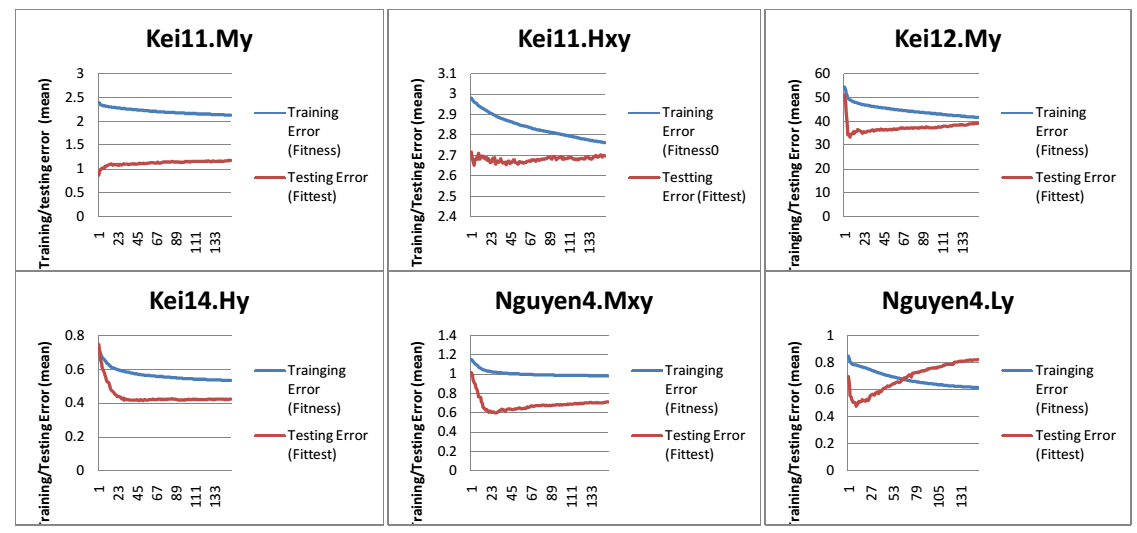
\includegraphics[scale=0.4]{Figures/Fig3_1.png}
% figure caption is below the figure
\caption{Some cases arise the first issues with the overfitting measurement proposed by Silva and colleagues.}
\label{fig:issue1}       % Give a unique label
\end{figure}

\item \textit{The second issue of detecting the best test point (btp)} \\ 
Correctly detecting the best test point will help us finding the generation where the overfitting issue starts to occur. This is very useful specifically to the early stopping of the GP learners. However, considering the case of the Nguyen4.Ly problem as shown in the Figure \ref{fig:issue2.1}, we see that this overfitting measure is also failed to capture the best test point correctly. The actual best test point ($btp_{actual}$) fount (at the $66^{th}$generation) is different from the expected best test point ($btp_{expected}$) (at generation $11^{th}$). The same issue (blocked while finding the $btp_{expected}$) caused by the condition (1) of this measure also occurs in cases as shown in the Figure \ref{fig:issue2.2}.

% For one-column wide figures use
\begin{figure}
% Use the relevant command to insert your figure file.
% For example, with the graphicx package use
\centering
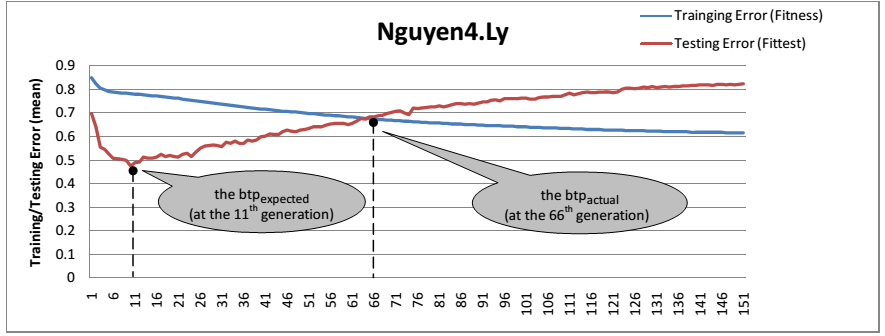
\includegraphics[scale=0.4]{Figures/Fig3_2.png}
% figure caption is below the figure
\caption{The case arises the second issue with the overfitting measurement proposed by Silva and colleagues.}
\label{fig:issue2.1}       % Give a unique label
\end{figure}

% For one-column wide figures use
\begin{figure}
% Use the relevant command to insert your figure file.
% For example, with the graphicx package use
\centering
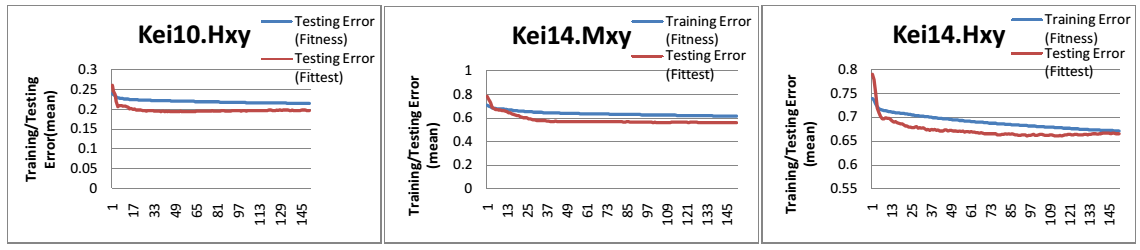
\includegraphics[scale=0.4]{Figures/Fig3_3.png}
% figure caption is below the figure
\caption{The more cases arise the second issue with the overfitting measurement proposed by Silva and colleagues.}
\label{fig:issue2.2}       % Give a unique label
\end{figure}


\subsubsection{The new overfitting measure}
In this section, we introduce a new overfitting method to overcome the limits of the overfitting measure proposed by Silva. The new method is based on this measure. Moreover, we also propose a new formula to quantifying the overfitting of the problem learned by GP. After that, we use it to measure the OV of benchmarks in our experiments. 
\begin{enumerate}
\item \textit{The new method to quantifying the OV at a generation}\\
The new method is built based on the method proposed by Silva as shown in the algorithm 1. Assuming that the best test point is at generation ${g}_{btp}$; $g$ is the current generation; $btp$ represents the best fittest error reached from when beginning of the  run until to the current generation. As shown in the algorithm 1, the amount of over-fitting at generation $g$ was calculated as follows (for more details, see the Figure \ref{fig:OV}):
\begin{eqnarray}
overfit(g)&=&{|training\_fit(g)-test\_fit(g)| - |tbtp-btp|} \nonumber\\
		  &=& {CF-AB}	\nonumber\\
          &=& {CF-DE}	\nonumber\\
		  &=& {|test\_fit(g) - btp|+|training\_fit(g)- tbtp|} \nonumber\\
		  &=& {CD+EF}  \nonumber\\
		  &=& {a_{g}+b_{g}}  \nonumber\\
\end{eqnarray}

% For one-column wide figures use
\begin{figure}
% Use the relevant command to insert your figure file.
% For example, with the graphicx package use
\centering
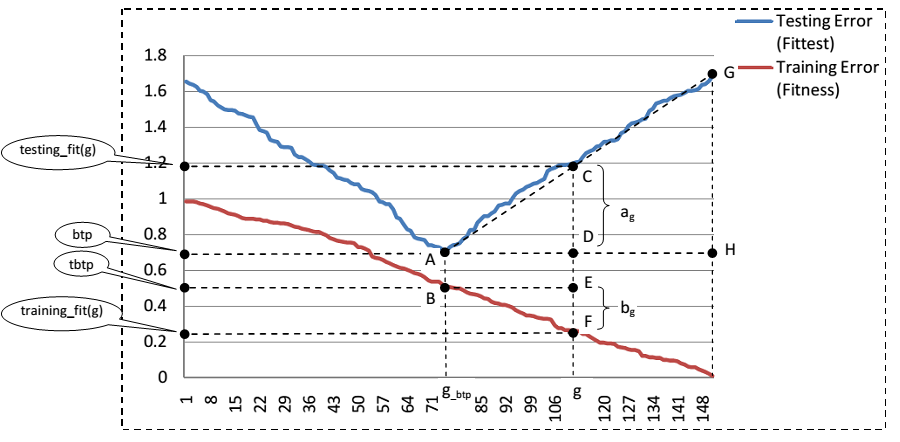
\includegraphics[scale=0.4]{Figures/Fig3_4.png}
% figure caption is below the figure
\caption{Graph for calculating the overfitting}
\label{fig:OV}       % Give a unique label
\end{figure}

We note that by using elitism mechanism in GP, so $training\_fit(g)$ is always less than or equal $tbtp$ at current generation $g$. Furthermore, in \cite{1996Mitchell}, the over-fitting be defined as follows:\textit{\textquotedblleft Given a hypothesis space $H$, a hypothesis $h \in H$ is said to overfit on the training sample if there exists some alternative hypothesis ${h}^{'} \in H$, such that $h$ has smaller error than ${h}^{'}$ over the training sample, but ${h}^{'}$ has smaller error than $h$ over the entire distribution of instances\textquotedblright}. This definition helps us not only find the best test point but also realize that the overfitting can be quantified independently to training error. So, in order to exactly reflect the amount of over-fitting at a generation, in the new overfitting formula, we eliminate the quantity of $b_{g}$. Therefore, the new measure to quantify the amount of over-fitting at generation $g$ now will be:
\begin{equation}
overfit (g) = a_{g} 	
\end{equation} \par
Besides, to overcome the issues that the Silva's method faced, We decide removing the condition (1) in this method. The details of our overfitting measure as shown in the algorithm 2 below.

\item \textit{The new method to quantify overfitting of problem} \\
Above, we mentioned the new overfitting measure at the generation g. In order to quantify the overfitting of a problem, beside considering the amount of over-fitting  at the final generation, we should consider more the early (or later) over-fitted characteristic of problem. In other words, the problem is overfitted early or lately need to quantify in this new method beside quantifying the overfitting at the final generation. So, the overfitting of problem should reflect two characteristics including the overfitting at the final generation and the generation that start be overfitted. This mean: the more over-fitting of a problem, the more overfitting at the final generation and the earlier over-fitting. To reflect these quantifies, we see the overfitting of the problem (OV) as a square root of a half of area of the triangle AGH (see the Figure \ref{fig:OV}), or 
\begin{equation}
OV=\sqrt{(a_{n}*(n-{g}_{btp}))/2} 
\end{equation}
where, $n$ is the number of generations; $btp$ is best test point be found after scanning from generation $1$ to generation $n$;  $a_{n}$ is the mount over-fitting at the final generation, n. The algorithm 2 presents details of this new method.
\begin{table}
\begin{tabular}{lllllllllll}
\multicolumn{11}{l}{\textbf{Algorithm 2}: The new overfitting measure} \\
\multicolumn{1}{l|}{} & \multicolumn{10}{l}{$overfit(0) = 0$} \\
\multicolumn{1}{l|}{} & \multicolumn{10}{l}{$btp = test\_fit(0)$} \\
\multicolumn{1}{l|}{} & \multicolumn{10}{l}{$tbtp = training\_fit(0)$} \\
\multicolumn{1}{l|}{} & \multicolumn{10}{l}{\textbf{for each } $generation$ $g>0$ } \\
\multicolumn{1}{l|}{} & \multicolumn{1}{l|}{} & \multicolumn{9}{l}{  \textbf{if} $(test\_fit(g) < btp)$} \\
\multicolumn{1}{l|}{} & \multicolumn{1}{l|}{} & \multicolumn{1}{l|}{} & \multicolumn{8}{l}{$overfit(g)= 0$} \\
\multicolumn{1}{l|}{} & \multicolumn{1}{l|}{} & \multicolumn{1}{l|}{} & \multicolumn{8}{l}{$btp = test\_fit(g)$} \\
\multicolumn{1}{l|}{} & \multicolumn{1}{l|}{} & \multicolumn{1}{l|}{} & \multicolumn{8}{l}{${g}_{btp}= g$} \\
\multicolumn{1}{l|}{} & \multicolumn{1}{l|}{} & \multicolumn{9}{l}{\textbf{else}} \\
\multicolumn{1}{l|}{} & \multicolumn{1}{l|}{} & \multicolumn{1}{l|}{} & \multicolumn{8}{l}{ $overfit(g) = |test\_fit(g) - btp| $} \\
\multicolumn{1}{l|}{} & \multicolumn{1}{l|}{} & \multicolumn{9}{l}{\textbf{endif}} \\
\multicolumn{1}{l|}{} & \multicolumn{10}{l}{\textbf{endfor}} \\
\multicolumn{1}{l|}{} & \multicolumn{10}{l}{$OV=\sqrt{overfit(n-1)*(n-{g}_{btp})/2}$ } \\
\multicolumn{1}{l|}{} & \multicolumn{10}{l}{\textbf{return} $OV$ } \\
\end{tabular}
\end{table}

\item \textit{Analyzing the effectiveness of the new overfitting measure}\\
By using our new method (see the algorithm 2), the discussed issues of Silva's overfitting method are solved. Considering the cases of problems as shown in the figure \ref{fig:issue1} and the figure \ref{fig:issue2.2} (Kei10.Hxy, Kei11.My, Kei11.Hxy, Kei12.My, Kei14.Hy, Kei14.Mxy, Kei14.Hxy, Nguyen4.Mxy, Nguyen4.Ly). The best test points corresponding with cases of problems are detected correctly by this new method, they occur at corresponding generations of 84, 0, 3, 6, 50, 106, 94, 27, 9. Besides, the corresponding overfitting values at the generations that start from ${g}_{btp}$ also be quantified.
\end{enumerate}
\end{enumerate}

\subsection {Grouping the problems based on over-fitting (OV)}
\label{clus}
After using the new overfitting measure to quantify the overfitting of problems, we use the \textit{Gene Cluster 3.0} software, a k-means clustering algorithm, to clustering these problems based on their overfitting. \textit{Gene Cluster 3.0} is the open source cluster software created by Michael Eisen and Seiya (University of Tokyo, Human Genome Center June 2002) and available at link:\\
\textit{http://www.mediafire.com/file/pdjzff1r7e5hx7f/clustersetup.exe}.

\section{Experimental setting}
\label{Exp}
\subsection{Benchmark problems}
\label{Ben}
As shown in \cite{2015Mig} not all functions are suitable to be used as benchmarks. Here, we choose Symbolic Regression functions from \cite{2012James} as shown in the Table \ref{tab:Problem}. Two reasons for selecting these functions are: (1) they did not receive any response from Genetic Programming community \cite{David2013}; (2) they have various response variable distributions to ensure the best coverage. In the Figure ~\ref{fig:Distribute}), shows response variable distributions of these functions: Kei12, Val5, Vla6, Nguyen\_1 are quite like Normal Distribution; functions like Kei10, Kei11, Vla1 with a few outliers in one tailed; Kei 15, Vla5 with more evenly outlier in both 2-tailed; functions as Kei14, Vla8, Nguyen\_2, Nguyen\_3, Nguyen\_4 with much higher density of outliers and very skew making them very challenging. \par
Towards a framework for synthetic problem generation shown in \cite{2015Mig}, all data sets generated from chosen functions have common features: input range, how to sample for the training and testing set, the number of samples in the testing set are the same in \cite{2012James}. However, because the size of training set could be used to analyze the difficulty of the problem \cite{2015Mig}. So to control the difficulty of the problem only through the measurement OV, we generate the training set with the  size of 200 samples for all functions. This size is recommended by Thomas and Lee Spector in \cite{Thomas2015}. They recommended that for most problems, training cases should be between 100 and 200, depending on the difficulty of the problem as well as the dimensionality of the input space.
%\begin{landscape}
\begin{table}
% table caption is above the table
\caption{GP Benchmark Regression Problems}
\label{tab:Problem}       % Give a unique label
% For LaTeX tables use
\begin{tabular}{llll}
\hline\noalign{\smallskip}
Name &  Definition & Training Data  & Testing Data\\
\noalign{\smallskip}\hline\noalign{\smallskip}
Kei10 &	 $x_{1}^{x_{2}}$ & U[0, 1, 200]	& E[0, 1, 0.01] \\
Kei11 & $x_{1}x_{2}+\sin((x_{1}-10)(x_{2}-1))$& U[-3, 3, 200] & E[-3, 3, 0.01] \\
Kei12 & $x_{1}^4-x_{1}^3+\frac{x_{2}^2}{2}-x_{2}$ & U[-3, 3, 200]	& E[-3, 3, 0.01] \\
Kei13 & $\sin(x_{1})\cos(x_{2})$ & U[-3, 3, 200]	& E[-3, 3, 0.01] \\
Kei14 & $\frac{8}{2+x_{1}^2+x_{2}^2}$ & U[-3, 3, 200]	& E[-3, 3, 0.01] \\
Kei15 & $\frac{x_{1}^3}{5}+\frac{x_{2}^3}{2}-x_{2}-x_{1}$ & U[-3, 3, 200]	& E[-3, 3, 0.01] \\
Vla1 & $\frac{{e^{{(x_{1}-1)}^2}}}{1.2+(x_{2}-2.5)^2}$ & U[0.3, 4, 200] & E[-0.2, 4.2, 0.01] \\
Vla5 & $30\frac{(x_{1}-1)(x_{3}-1)}{x_{2}^2(x_{1}-10)}$ &
$\begin{array}{l} x_{1}: \textnormal{U}[0.05, 2, 200] \\ %U khong bi nghieng
x_{2}: \textnormal{U}[1, 2, 200]\\
x_{3}: \textnormal{U}[0.05, 2, 200] \end{array}$	& $\begin{array}{l} x_{1}: \textnormal{E}[-0.05, 2.1, 0.15]\\
x_{2}: \textnormal{E}[0.95, 2.05, 0.1] \\
x_{3}: \textnormal{E}[-0.05, 2.1, 0.15] \end{array} $\\
Vla6 & $6\sin(x_{1})\cos(x_{2})$ & U[0.1, 5.9, 200] & E[-0.05, 6.05, 0.02] \\
Val8 & $\frac{(x_{1}-3)^4+(x_{2}-3)^3-(x_{2}-3)}{(x_{2}-2)^4+10}$ & U[0.05, 6.05, 200] &	E[-0.25, 6.35, 0.2] \\
Nguyen\_1 & $ x^3+x^2+x $ & U[-1,1,200] & U[-1,1,100] \\
Nguyen\_2 & $ x^4+x^3+x^2+x $ & U[-1,1,200]	& U[-1,1,100] \\
Nguyen\_3 & $ x^5+x^4+x^3+x^2+x $ & U[-1,1,200]	& U[-1,1,100] \\
Nguyen\_4 & $ x^6+x^5+x^4+x^3+x^2+x $ & U[-1,1,200]	& U[-1,1,100] \\
\noalign{\smallskip}\hline
\end{tabular}
\end{table}
%\end{landscape}

% For one-column wide figures use
\begin{figure}
% Use the relevant command to insert your figure file.
% For example, with the graphicx package use
\centering
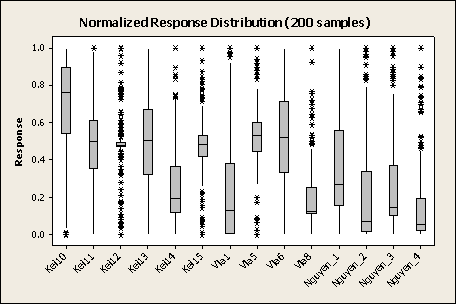
\includegraphics[scale=0.6]{Figures/Figure3.png}
% figure caption is below the figure
\caption{Normalized response variable distribution over 200 samples for each function (response variable normalized by the formula in \cite{2015Mig})}
\label{fig:Distribute}       % Give a unique label
\end{figure}
\subsection{GP Parameters Setting}
\label{GPP}
The GP parameters used for our experiments are shown in the Table \ref{tab:Parameter}. These are typical settings often used by GP researchers and practitioners \cite{1992Koza}. However, to stabilize the variance of the intermediate quantities in the individual tree we use an analytic quotient (AQ) operator \cite{Ni2013} instead of the protected division (PD).
\begin{table}
% table caption is above the table
\caption{Run and Evolutionary Parameters Values}
\label{tab:Parameter}       % Give a unique label
% For LaTeX tables use
\begin{tabular}{ll}
\hline\noalign{\smallskip}
Parameter & Value \\
\noalign{\smallskip}\hline\noalign{\smallskip}
Problems &	Shown in the Table \ref{tab:Problem}  \\
EA used in GP systems &	Elitist, generational, expression tree representation \\
Function set &	+, -, *, / (AQ) \\
Terminal set &	Regression variables and one random constant in [0.0, 1.0] \\
No. of generations	& 151 \\
Population size	& 500 \\
Tournament size &	4 \\
Tree creation	& Ramped half-and-half (depths of 2 to 6) \\
Max. tree depth	& 15 \\
Sub tree crossover rate	& 0.9 \\
Sub tree mutation rate & 0.1 \\
No.  of Runs & 51 \\
Fitness function & RMSE \\
\noalign{\smallskip}\hline
\end{tabular}
\end{table}
\section {Results and discussion}
\label{Res}
In this section we present the experimental results of running GP with all noise configurations for all chosen benchmarks. Experimental results include: OV of the best learned model as shown in the Table \ref{tab:OV}; generalization errors; complexities of the best model, all is averaged over 51 runs, as shown in the Table \ref{tab:Fittest}, the Table \ref{tab:size}.
\subsection {Grouping generated data sets by over-fitting (OV)}
\label{Gro}
Table \ref{tab:OV} shows 140 data sets grouped to four clusters by their OVs. Each cluster includes benchmarks with OVs are increasing. The clustering results are shown in the Table \ref{tab:cluster}, the Table \ref{tab:InfCluster}.  To cluster, we used the k-means clustering algorithm as mentioned at section \ref{clus}. With this k-means clustering algorithm, we select the Euclidean distance,  repeat 100 times and use of median rather than mean centering, due to it is more robust against outliers. We can download data sets and the reference table providing detailed information for each data set in folder \textquotedblleft data Sets\textquotedblright at address:\\ \textit{https://www.dropbox.com/s/udek9c9ww44cjbu/Data\%20sets.rar?dl=0}
%\begin{landscape}
\begin{table}
% table caption is above the table
\caption{Four groups of generated data sets were clustered by criteria OV}
\label{tab:cluster}       % Give a unique label
% For LaTeX tables use
%a) Four groups of data sets were clustered by criteria OV
\begin{tabular}{lllll}
%\multicolumn{6}{l}{a) Four groups of generated data sets were clustered by criteria OV} \\
\hline\noalign{\smallskip}
& \multicolumn{4}{c}{Name of data set (Index of data set)} \\
\noalign{\smallskip}\hline\noalign{\smallskip}
& Kei2.My & Kei12.Ly & Kei12.Hy & Kei12.Hxy \\
Cluster 0 & Kei12.Hx & Kei12.Mx & Nguyen\_4.Ly & Kei11.My \\
(C0) & Kei11.Ly & Nguyen\_4.Hy & Kei11.Lxy & Vla1.Hx \\
& Nguyen\_4.Hx & & & \\
\hline
& Vla1.Lxy & Nguyen\_4.My & Kei12.Lx & Vla8.My \\
& Vla1.Hy & Nguyen\_4.Lx & Kei10.Hy & Nguyen\_3.Mxy \\
& Vla5.Lxy & Kei13.Hy & Kei14.Mxy & Vla8.Hxy \\
& Vla8.Hy & Vla6.Mx & Kei14.Lx & Vla8.Mx \\
& Kei10.Mxy & Kei13.My & Vla1.Mx & Kei13.My \\
& Vla6.My & Nguyen\_4.Mx & Vla6.Hy & Kei13.Mxy \\
Cluster 1 & Nguyen\_2.Mx & Vla5.My & Nguyen\_2.Ly & Kei13.Ly \\
(C1) & Vla1.Lx & Vla1.Ly & Vla6.Ly & Kei15.Mx \\
& Vla8.Lx & Kei10.Mx & Kei10.Ly & Kei10.Ly \\
& Kei14.Lxy & Kei10.Lxy & Kei10.F & Kei11.F \\
& Kei12.F & Kei13.F & Kei14.F & Kei15.F \\
& Vla1.F & Vla5.F & Vla6.F & Vla8.F \\
& Nguyen\_1.tr10 & Nguyen\_2.F & Nguyen\_3.F & Nguyen\_4. F \\
& Kei13.Lx & Kei15.Lx & Vla6.Lx & Nguyen\_3.Ly \\
& Vla5.Ly & Vla8.Ly & Vla6.Lxy & Vla8.Lxy \\
& Nguyen\_1.Lxy & Vla6.Mxy & Nguyen\_1.Mxy & \\
\hline
& Nguyen\_1.My & Kei14.My & Vla5.Hy & Nguyen\_4.Lxy \\
& Kei15.Hx & Kei11.Mxy & Kei14.Hy & Kei14.Ly \\
& Nguyen\_2.Lx & Vla5.Hxy & Vla6.Hxy & Kei14.Hx \\
& Vla8.Hx & Kei14.Mx & Nguyen\_1.Hx & Vla1.My \\
Cluster 2 & Vla5.Mxy & Nguyen\_1.Mx & Nguyen\_2.Hxy & Nguyen\_3.Mx\\
(C2) & Kei10.Hxy & Nguyen\_1.Hxy & Kei14.Hxy & Vla6.Hx \\
& Kei15.Lxy & Kei13.Hx & Kei10.Hx & Vla5.Hx \\
& Vla1.Hxy & Kei15.Ly  & Nguyen\_2.Lxy & Vla5.Lx \\
& Kei10.My & Vla5.Mx & Vla1.Mxy & Kei13.Lxy \\
& Nguyen\_3.Lxy & Kei12.Lxy & & \\
\hline
& Kei11.Hy & Nguyen\_3.Hy & Nguyen\_4.Hxy & Nguyen\_4.Mxy \\
& Kei11.Mx & Nguyen\_2.Hy & Kei12.Mxy & Kei15.Hy \\
Cluster 3 & Kei11.Lx & Kei11.Hxy & Nguyen\_2.Mxy & Kei15.Mxy \\
(C3) & Nguyen\_2.My & Nguyen\_3.Ly & Nguyen\_3.Hx & Nguyen\_1.Ly \\
& Kei15.My & Nguyen\_3.My & Nguyen\_1.Lx & Nguyen\_1.Hy \\
& Vla8.Mxy & Kei13.Hxy & Nguyen\_2.Hx & Nguyen\_3.Hxy \\
& Kei15.Hxy & Kei11.Hx & & \\

\noalign{\smallskip}\hline
\end{tabular}
\end{table}
%b) clustering information \\
\begin{table}
% table caption is above the table
\caption{ Information of clusters}
\label{tab:InfCluster}       % Give a unique label
\begin{tabular}{lllll}
%\multicolumn{5}{l}{b) clustering information} \\
\hline\noalign{\smallskip}
& Cluster 0 & Cluster 1 & Cluster 2 & Cluster 3 \\
\noalign{\smallskip}\hline\noalign{\smallskip}
No. of observations	& 13 &	63 &	38 &	26 \\
Within cluster sum of squares &	592.7936 &	0.28177 &	1.447554	& 11.98758 \\
Average distance from centroid &	4.256253 &	 0.049527	& 0.146812 &	0.527065 \\
Max distance from centroid	& 15.390471 &	0.168109 &	0.453639 &	1.491932 \\
Cluster centroids &	4.949519	& 0.021502 &	0.386764 &	1.385605 \\
Distances between centroids  & $\begin{array}{l}  C0 \rightarrow C1:\\
4.928017 \\
C0 \rightarrow C2:\\
4.562755 \\
C0 \rightarrow C3:\\
3.563914 \end{array}$ & $\begin{array}{l} C1 \rightarrow C2:\\
0.365262 \\
C1 \rightarrow C3:\\
1.364103 \end{array}$ & $\begin{array}{l} C2 \rightarrow C3:\\
0.998841 \end{array}$ & \\
OV range: [min, max] & $\begin{array}{l}	[3.186061,\\
20.33999] \end{array}$ & $\begin{array}{l}	[0,\\
0.189611]\end{array}$ & $\begin{array}{l} [0.208218,\\
0.841303] \end{array}$ & $\begin{array}{l} [0.913296, \\ 2.877537] \end{array}$\\
OV level &	High &	Free &	Low	& Medium \\
\noalign{\smallskip}\hline
\end{tabular}
\end{table}
%\end{landscape}

%\begin{landscape}
\begin{center}
\begin{table}
% table caption is above the table
\caption{Mean of OVs of the best model trained on generated data sets using the formula (3)}
\label{tab:OV}       % Give a unique label
% For LaTeX tables use
\begin{tabular}{lllllllllll}
\hline\noalign{\smallskip}
& F & Lx & Mx & Hx & Ly & My & Hy & Lxy & Mxy & Hxy  \\
\noalign{\smallskip}\hline\noalign{\smallskip}
Kei10 & 0 & 0.01 & 0.01 & 0.30 & 0.01 & 0.26 & 0.14 & 0.00 & 0.09 & 0.37 \\
Kei11 & 0 & 1.89 & 2.44 & 0.91 & 4.40 & 4.82 & 2.88 & 3.99 & 0.71 & 1.82 \\
Kei12 & 0 & 0.18 & 4.96 & 9.31 & 18.70 & 20.34 & 15.10 & 0.21 & 2.03 & 11.13 \\
Kei13 & 0 & 0.00 & 0.09 & 0.31 & 0.04 & 0.09 & 0.13 & 0.24 & 0.06 & 1.04 \\
Kei14 & 0 & 0.10 & 0.43 & 0.51 & 0.65 & 0.82 & 0.68 & 0.01 & 0.12 & 0.36 \\
Kei15 & 0 & 0.00 & 0.02 & 0.71 & 0.28 & 1.21 & 1.96 & 0.33 & 1.74 & 1.00 \\
Vla1 & 0 & 0.04 & 0.09 & 3.70 & 0.04 & 0.43 & 0.16 & 0.19 & 0.24 & 0.30 \\
Vla5 & 0 & 0.26 & 0.25 & 0.30 & 0.00 & 0.05 & 0.81 & 0.13 & 0.41 & 0.59 \\
Vla6 & 0 & 0.00 & 0.10 & 0.34 & 0.04 & 0.08 & 0.06 & 0.00 & 0.00 & 0.52 \\
Vla8 & 0 & 0.01 & 0.10 & 0.44 & 0.00 & 0.17 & 0.11 & 0.00 & 1.10 & 0.11 \\
Nguyen\_1 & 0 & 1.12 & 0.40 & 0.43 & 1.28 & 0.84 & 1.10 & 0.00 & 0.00 & 0.37 \\
Nguyen\_2 & 0 & 0.65 & 0.05 & 1.03 & 0.05 & 1.40 & 2.29 & 0.28 & 1.75 & 0.39 \\
Nguyen\_3 & 0 & 0.00 & 0.38 & 1.30 & 1.37 & 1.15 & 2.79 & 0.21 & 0.14 & 1.02 \\
Nguyen\_4 & 0 & 0.15 & 0.08 & 3.19 & 4.95 & 0.19 & 4.12 & 0.78 & 2.63 & 2.72 \\


\noalign{\smallskip}\hline
\end{tabular}
\end{table}
\begin{table}
% table caption is above the table
\caption{Fittest (mean) of the best learned model by GP with noise configurations}
\label{tab:Fittest}       % Give a unique label
% For LaTeX tables use
\begin{tabular}{lllllllllll}
\hline\noalign{\smallskip}
Problem & F & Lx & Mx & Hx & Ly & My & Hy & Lxy & Mxy & Hxy  \\
\noalign{\smallskip}\hline\noalign{\smallskip}
Kei-10 & 0.05 & 0.08 & 0.12 & 0.17 & 0.07 & 0.10 & 0.16 & 0.07 & 0.16 & 0.20 \\
Kei-11 & 0.56 & 0.91 & 1.66 & 2.33 & 0.96 & 1.18 & 1.56 & 1.03 & 2.47 & 2.70 \\
Kei-12 & 1.83 & 24.0 & 31.2 & 45.8 & 18.8 & 39.2 & 40.4 & 14.7 & 45.2 & 56.0 \\
Kei-13 & 0.67 & 1.41 & 2.05 & 2.34 & 0.96 & 1.68 & 2.19 & 1.35 & 2.60 & 2.70 \\
Kei-14 & 0.10 & 0.22 & 0.32 & 0.59 & 0.19 & 0.27 & 0.42 & 0.35 & 0.56 & 0.67 \\
Kei-15 & 0.73 & 0.97 & 1.68 & 2.44 & 1.43 & 1.46 & 2.55 & 1.39 & 2.56 & 3.19 \\
Vla-1 & 0.07 & 0.07 & 0.10 & 1.86 & 0.09 & 0.11 & 0.12 & 0.08 & 0.13 & 0.19 \\
Vla-5 & 0.34 & 0.44 & 0.66 & 0.62 & 0.36 & 0.47 & 0.65 & 0.53 & 0.75 & 0.74 \\
Vla-6 & 1.99 & 2.10 & 2.54 & 2.66 & 2.09 & 2.22 & 2.39 & 2.19 & 2.45 & 2.80 \\
Vla-8 & 1.12 & 1.59 & 1.89 & 2.17 & 1.33 & 1.51 & 2.13 & 1.61 & 2.10 & 2.26 \\
Nguyen-1 & 0.00 & 0.12 & 0.28 & 0.32 & 0.13 & 0.30 & 0.49 & 0.12 & 0.45 & 0.61 \\
Nguyen-2 & 0.01 & 0.06 & 0.17 & 0.47 & 0.11 & 0.29 & 0.72 & 0.17 & 0.42 & 0.50 \\
Nguyen-3 & 0.01 & 0.05 & 0.29 & 0.47 & 0.13 & 0.44 & 0.80 & 0.24 & 0.64 & 0.68 \\
Nguyen-4 & 0.02 & 0.14 & 0.65 & 0.93 & 0.82 & 0.58 & 1.09 & 0.54 & 0.71 & 1.49 \\
Mean & 0.53 & 2.30 & 3.11 & 4.51 & 1.96 & 3.56 & 3.97 & 1.74 & 4.37 & 5.34 \\

\noalign{\smallskip}\hline
\end{tabular}
\end{table}

\begin{table}
% table caption is above the table
\caption{Model complexity (mean) of the best learned model by GP with noise configurations}
\label{tab:size}       % Give a unique label
% For LaTeX tables use
\begin{tabular}{lllllllllll}
\hline\noalign{\smallskip}
Problem & F & Lx & Mx & Hx & Ly & My & Hy & Lxy & Mxy & Hxy  \\
\noalign{\smallskip}\hline\noalign{\smallskip}
Kei-10 & 270 & 311 & 338 & 348 & 288 & 315	& 338 &	331	& 309 & 288 \\
Kei-11 & 348 & 349 & 360 & 387 & 399 & 352 & 377 & 364 & 405 & 420 \\
Kei-12 & 291 & 408 & 473 & 442 & 381 & 414 & 428 & 376 & 447 & 531 \\
Kei-13 & 355 & 377 & 440 & 422 & 378 & 383 & 401 & 356 & 447 & 420 \\
Kei-14 & 205 & 261 & 276 & 284 & 259 & 257 & 270 & 258 & 262 & 271 \\
Kei-15 & 311 & 338 & 328 & 394 & 346 & 355 & 389 & 332 & 391 & 396 \\
Vla-1 & 328 & 312 & 341 & 324 & 339 & 337 & 359 & 329 & 324 & 342 \\
Vla-5 & 278 & 361 & 362 & 400 & 324 & 346 & 380 & 357 & 442 & 425 \\
Vla-6 & 399 & 410 & 410 & 389 & 391 & 414 & 428 & 415 & 415 & 407 \\
Vla-8 & 381 & 391 & 358 & 338 & 373 & 372 & 334 & 371 & 337 & 315 \\
Nguyen-1 & 159 & 331 & 406 & 402 & 354 & 380 & 380 & 396 & 411 & 453 \\
Nguyen-2 & 220 & 331 & 481 & 420 & 351 & 385 & 476 & 405 & 410 & 408 \\
Nguyen-3 & 245 & 288 & 382 & 406 & 381 & 405 & 390 & 365 & 423 & 435 \\
Nguyen-4 & 254 & 304 & 423 & 442 & 472 & 404 & 425 & 432 & 432 & 482 \\
Kei-10 & 426 & 411 & 420 & 449 & 405 & 427 & 361 & 403 & 411 & 476 \\
\noalign{\smallskip}\hline
\end{tabular}
\end{table}
\end{center}
%\end{landscape}

\subsection {Analysis of the robustness of GP to noise}
\label{AnaFittest}
Experimental results show that for all three noise types: noise x, noise y, noise x \& y: the more noise, the greater fittest error) of the best solution (see the cases in bold in the Table \ref{tab:Fittest}) with most of benchmark functions. To be more clear, we can observe fittest error of the best model over the generations with the noise configurations in the Figure \ref{fig:Fittest}. The cause can be the higher noise levels and would make the problem more difficult to learn exact models. For example, fitness errors of some functions shown in the Figure ~\ref{fig:Fitness} (graph of all functions can see in https://www.dropbox.com/s/gnuinkzicoq9jdr/Graph.rar?dl=0) clearly state that: fitness error of the best model with noise levels of 0\% noise is smaller than with 10\% noise ($finess(0 \%) < fitness(10\%)$); similarly, $finess(10\%) < fitness(30\%)$; $fitness(30\%) < fitness(50\%)$. \par
The greater noise level (with all three types of noise) not only make the generalization ability reduced but also increase the complexity of learned models with most of problems (see the Table \ref{tab:size}). Thus, we can conclude GP is not powerful Machine Learning technique with noise.
\begin{figure}
% Use the relevant command to insert your figure file.
% For example, with the graphicx package use
  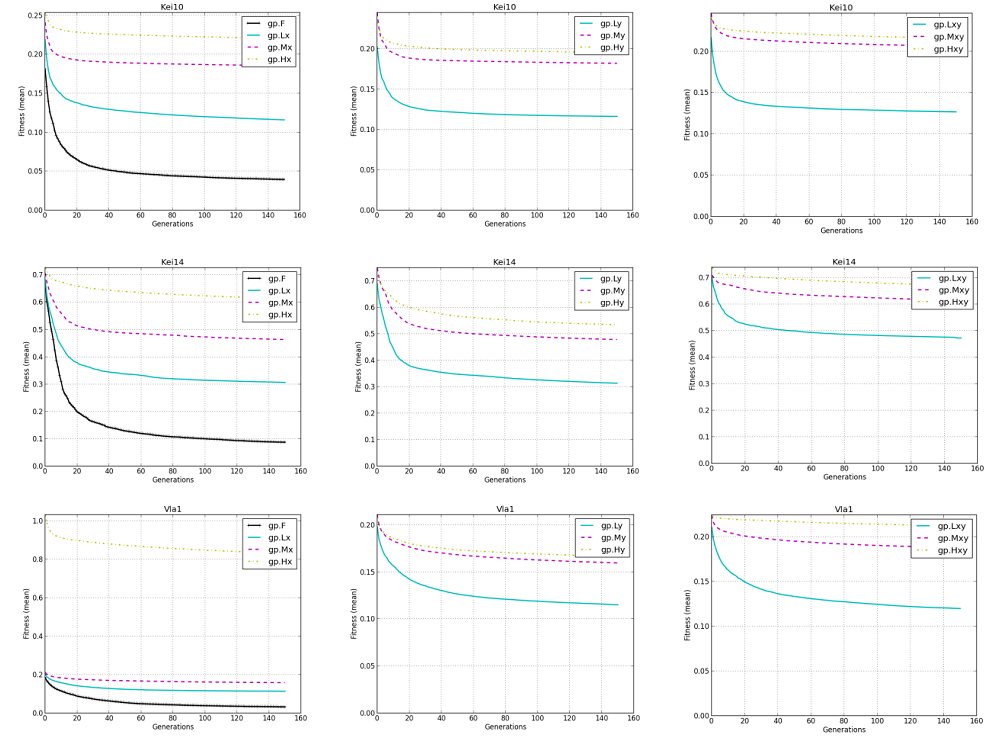
\includegraphics[width=1.0\textwidth]{Figures/Figure4.png}
  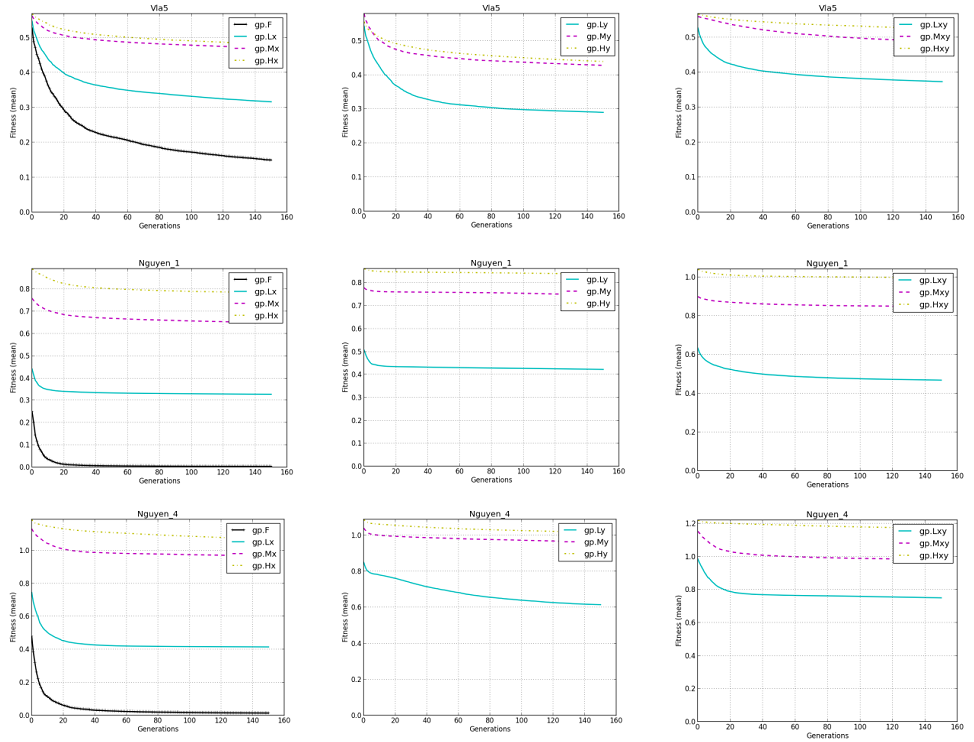
\includegraphics[width=1.0\textwidth]{Figures/Figure5.png}
 % figure caption is below the figure
\caption{Fitness (mean) of the best learned model by GP with noise configurations}
\label{fig:Fitness}       % Give a unique label
\end{figure}
\begin{figure}
% Use the relevant command to insert your figure file.
% For example, with the graphicx package use
  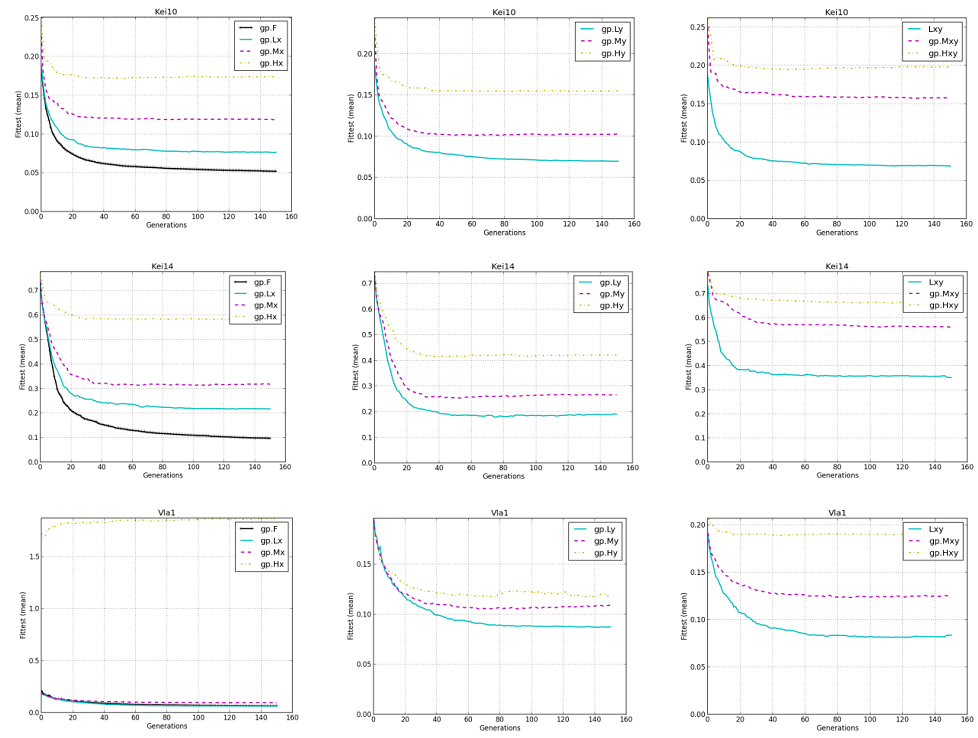
\includegraphics[width=1.0\textwidth]{Figures/Figure7.png}
  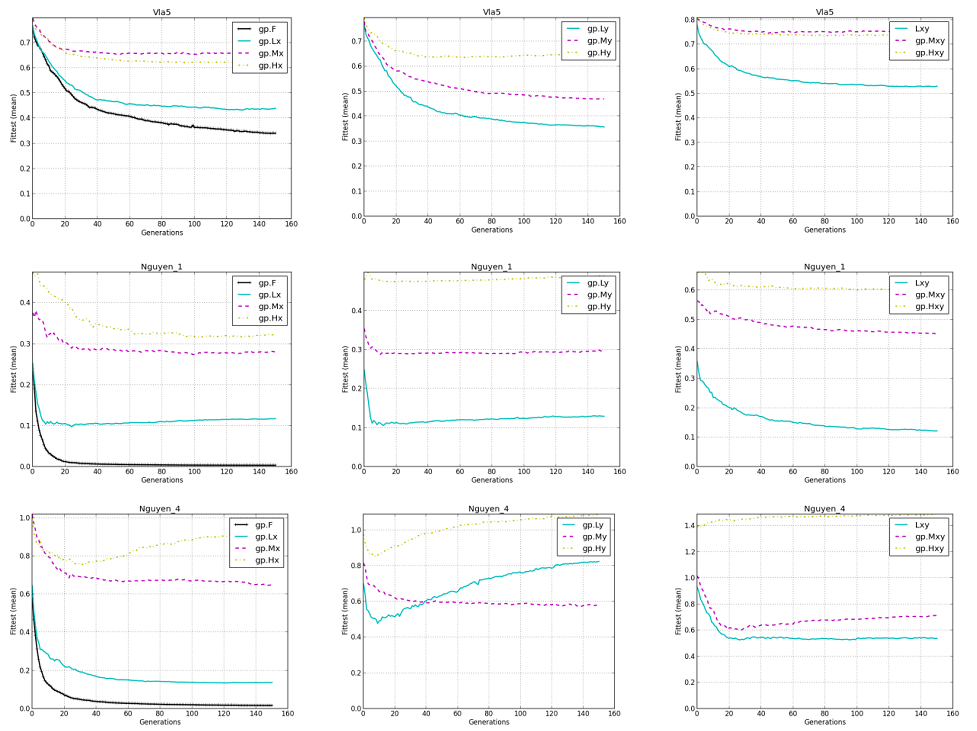
\includegraphics[width=1.0\textwidth]{Figures/Figure8.png}
 % figure caption is below the figure
\caption{Fittest (mean) of the best learned model by GP with noise configurations}
\label{fig:Fittest}       % Give a unique label
\end{figure}
\subsection {Analysis of the differences between the noise types, noise levels}
\label{AnaDiff}
Beside some common features as shown in the section \ref{AnaFittest}, each noise type, each noise level has has a few distinct characteristics from: (1) the magnitude of fittest error; (2) the convergence rate; (3) the over-fitted ability of solutions. To show the difference we use a function: sign(x): returns (+) if $x>0$ else returns (-).
\subsubsection{The differences in the magnitude of fittest error}
\label{AnaDiffMag}
Most of the problems with the same noise level, the same function, the fittest error of solutions that training on data set added noise x,y is often less than on data set added noise xy:
\begin{itemize}
\item Consider the cases of noise x and noise xy: with most of benchmark functions, fittest error of the best model on original data with noise x is often less than with noise xy. In the Table \ref{tab:difFittest}, the negative (-) cases show the fittest error with noise xy is less than with. At the level of noise by 10\%, there are 11 from 14 functions include: Kei11, Kei14, Kei15, Vla1, Vla5, Vla6, Vla8, Nguyen\_1, Nguyen\_2, Nguyen\_3 and Nguyen-4 (11/14 functions). There are 13/14; 13/14 functions corresponding to levels of noise 30\%; 50\%.
\item Consider the case of noise y and noise xy: there are 8/14, 14/14, 12/14 functions at the noise level of 10\%, 30\%, 12\%,respectively. Their fittest errors with noise x are less than with noise xy.
\item Consider the case of noise x and noise y. The difference is not clear. The number of problems that noise x give fittest error greater than noise y are 7/14; 5/14; 6/14 corresponding to the levels of noise by 10\%; 30\%; 50\%.
\end{itemize} \par
%\begin{landscape}
\begin{table}
\caption{The difference (result of subtracting fittest errors) in the fittest error of the best model with various noise types: (a) sign(Fittest(Noise x) - Fittest(Noise y)); (b) sign(Fittest(Noise x) - Fittest(Noise xy)); c) sign(Fittest(noise y)-Fittest(noise xy)}
\label{tab:difFittest}       % Give a unique label
\begin{tabular}{l|lll|lll|lll}
\hline\noalign{\smallskip}
Problem & \multicolumn{3}{c|}{(a)} & \multicolumn{3}{c|}{(b)} & \multicolumn{3}{c}{(c)} \\
 & \multicolumn{1}{c}{\textit{10\%}} & \multicolumn{1}{c}{\textit{30\%}} & \multicolumn{1}{c|}{\textit{50\%}} & \multicolumn{1}{c}{\textit{10\%}} & \multicolumn{1}{c}{\textit{30\%}} & \multicolumn{1}{c|}{\textit{50\%}} & \multicolumn{1}{c}{\textit{10\%}} & \multicolumn{1}{c}{\textit{30\%}} & \multicolumn{1}{c}{\textit{50\%}} \\
\hline
Kei10 & + & + & + & + & - & - & + & - & - \\
Kei11 & - & + & + & - & - & - & - & - & - \\
Kei12 & + & - & + & + & - & - & + & - & - \\
Kei13 & + & + & + & + & - & - & - & - & - \\
Kei14 & + & + & + & - & - & - & - & - & - \\
Kei15 & - & + & - & - & - & - & + & - & - \\
Vla1 & - & - & + & - & - & + & + & - & - \\
Vla5 & + & + & - & - & - & - & - & - & - \\
Vla6 & + & + & + & - & + & - & - & - & - \\
Vla8 & + & + & + & - & - & - & - & - & - \\
Nguyen\_1 & - & - & - & - & - & - & + & - & - \\
Nguyen\_2 & - & - & - & - & - & - & - & - & + \\
Nguyen\_3 & - & - & - & - & - & - & - & - & + \\
Nguyen\_4 & - & + & - & - & - & - & + & - & - \\
\hline
\end{tabular}
\end{table}
\subsubsection {The differences in the convergence rate}
\label{AnaDiffCR}
To explore different effects of noise to the speed of convergence of the best solution, we calculated the mean of convergence speed over generations by taking fitness error of previous generation minus this error of later generation and cumulative, then averaged. The results shown in the Table \ref{tab:CR}. \par
Results in the Table \ref{tab:CR} give us comments: (1) With the same noise type, the converging rate decreased when the noise increased on most of benchmark functions. More clearly, we can see the Table \ref{tab:difCR1} is built from the Table \ref{tab:CR} in which cells with sign (+) indicate $CR(0\% noise) > CR(10\% noise)$ ;$ CR(10\%) > CR(30\%)$ and $ CR(30\%) > CR(50\%)$, it is true for all noise types; (2) see the Table \ref{tab:difCR2} most of functions, with the same level of noise, the convergence rate of the best model on the data set with noise x, y is larger than on the data set with noise xy, especially when the noise increased. However, this distinction is not clear between noise x and noise y:
\begin{enumerate}
\item Considering the case of noise x and noise xy:
\begin{enumerate}
\item At the level of noise by 10\%, there are 9 functions from 14 benchmark functions: Kei10, Kei11, Kei14, Kei15, Vla1, Vla5, Vla6 Nguyen-3, Nguyen-4 have $CR(noise x) > CR(noise xy)$.
\item At the level of noise by 30\%, all benchmark  functions  (except Kei11, Vla6, Nguyen-4) have $CR(noise x) > CR(noise xy)$ (11/14 functions).
\item At the level of noise by 50\%, all benchmark  functions have $ CR(noise x) > CR(noise xy)$ (14/14 functions).
\end{enumerate}
\item Considering the case of noise y and noise xy: At the levels of noise by 10\%, 30\%, 50\%, respectively, there are 8/14, 10/14, 13/14 functions which the convergence rate of the best learned model on data set with noise y is greater than on data set with noise xy.
\item Considering the case of noise x and noise y, the difference is not clear. At the levels of noise by 10\%, 30\%, 50\%, respectively, there are 8/14, 7/14, 7/14 functions which the converging rate of the best model on data set added noise x is greater than on data set added noise y.
\end{enumerate} \par
\begin{table}
% table caption is above the table
\caption{Mean of the convergence rate across generations (measured through the fitness error of the best model)}
\label{tab:CR}       % Give a unique label
% For LaTeX tables use
\begin{tabular}{lllllllllll}
\hline\noalign{\smallskip}
Problem & F & Lx & Mx & Hx & Ly & My & Hy & Lxy & Mxy & Hxy  \\
\noalign{\smallskip}\hline\noalign{\smallskip}
Kei10 & 9.E-04 & 7.E-04 & 4.E-04 & 2.E-04 & 6.E-04 & 4.E-04 & 3.E-04 & 6.E-04 & 3.E-04 & 2.E-04 \\
Kei11 & 1.E-03 & 4.E-03 & 2.E-03 & 2.E-03 & 2.E-03 & 2.E-03 & 2.E-03 & 2.E-03 & 2.E-03 & 1.E-03 \\
Kei12 & 3.E-01 & 2.E-01 & 1.E-01 & 7.E-02 & 2.E-01 & 8.E-02 & 6.E-02 & 2.E-01 & 6.E-02 & 4.E-02 \\
Kei13 & 1.E-02 & 6.E-03 & 3.E-03 & 2.E-03 & 9.E-03 & 5.E-03 & 2.E-03 & 7.E-03 & 2.E-03 & 2.E-03 \\
Kei14 & 4.E-03 & 3.E-03 & 2.E-03 & 8.E-04 & 3.E-03 & 2.E-03 & 1.E-03 & 2.E-03 & 7.E-04 & 5.E-04 \\
Kei15 & 9.E-03 & 8.E-03 & 3.E-03 & 2.E-03 & 6.E-03 & 4.E-03 & 3.E-03 & 5.E-03 & 2.E-03 & 2.E-03 \\
Vla1 & 1.E-03 & 6.E-04 & 4.E-04 & 1.E-03 & 6.E-04 & 4.E-04 & 3.E-04 & 6.E-04 & 3.E-04 & 9.E-05 \\
Vla5 & 3.E-03 & 2.E-03 & 6.E-04 & 6.E-04 & 2.E-03 & 1.E-03 & 8.E-04 & 1.E-03 & 5.E-04 & 3.E-04 \\
Vla6 & 8.E-03 & 5.E-03 & 2.E-03 & 2.E-03 & 5.E-03 & 4.E-03 & 3.E-03 & 4.E-03 & 2.E-03 & 1.E-03 \\
Vla8 & 6.E-03 & 3.E-03 & 2.E-03 & 1.E-03 & 4.E-03 & 3.E-03 & 1.E-03 & 4.E-03 & 1.E-03 & 4.E-04 \\
Nguyen\_1 & 2.E-03 & 8.E-04 & 7.E-04 & 7.E-04 & 6.E-04 & 2.E-04 & 2.E-04 & 1.E-03 & 4.E-04 & 3.E-04 \\
Nguyen\_2 & 2.E-03 & 1.E-03 & 2.E-03 & 4.E-04 & 8.E-04 & 4.E-04 & 2.E-04 & 1.E-03 & 8.E-04 & 4.E-04 \\
Nguyen\_3 & 3.E-03 & 2.E-03 & 1.E-03 & 1.E-03 & 1.E-03 & 7.E-04 & 7.E-04 & 2.E-03 & 6.E-04 & 5.E-04 \\
Nguyen\_4 & 3.E-03 & 2.E-03 & 1.E-03 & 8.E-04 & 2.E-03 & 5.E-04 & 5.E-04 & 2.E-03 & 1.E-03 & 3.E-04 \\
\noalign{\smallskip}\hline
\end{tabular}
\end{table}
%\end{landscape}
\begin{table}
% table caption is above the table
\caption{The difference in the convergence rate (CR) of the best model on the data sets have the same type of noise but various noise levels: (a) sign(CR(0\%)- CR(10\%)); (b) sign(CR(10\%)- CR(30\%)); (c) sign(CR(30\%)- CR(50\%)) }
\label{tab:difCR1}       % Give a unique label
% For LaTeX tables use
\begin{tabular}{l|lll|lll|lll}
\hline\noalign{\smallskip}
Problem & \multicolumn{3}{c|}{Noise x} & \multicolumn{3}{c|}{Noise y} & \multicolumn{3}{c}{Noise xy} \\
 & (a) & (b) & (c) & (a) & (b) & (c) & (a) & (b) & (c) \\
\noalign{\smallskip}\hline\noalign{\smallskip}
Kei10 & + & + & + & + & + & + & + & + & + \\
Kei11 & - & + & - & - & - & - & - & - & + \\
Kei12 & + & + & + & + & + & + & + & + & + \\
Kei13 & + & + & + & + & + & + & + & + & + \\
Kei14 & + & + & + & + & + & + & + & + & + \\
Kei15 & + & + & + & + & + & + & + & + & - \\
Vla1 & + & + & - & + & + & + & + & + & + \\
Vla5 & + & + & + & + & + & + & + & + & + \\
Vla6 & + & + & + & + & + & + & + & + & + \\
Vla8 & + & + & + & + & + & + & + & + & + \\
Nguyen\_1 & + & + & + & + & + & + & + & + & + \\
Nguyen\_2 & + & - & + & + & + & + & + & + & + \\
Nguyen\_3 & + & + & - & + & + & + & + & + & + \\
Nguyen\_4 & + & + & + & + & + & + & + & + & + \\
\noalign{\smallskip}\hline
\end{tabular}
\end{table}
\begin{table}
\caption{The difference in the convergence rate (CR) of the best model on the data sets have the same noise level but various noise types: (a) sign(CR (noise x) - CR (noise y)); (b) sign(CR (noise x) - CR (noise xy)); (c) sign(CR (noise y) - CR (noise xy))}
\label{tab:difCR2}
\begin{tabular}{l|lll|lll|lll}
\hline\noalign{\smallskip}
Problem & \multicolumn{3}{c|}{(a)} & \multicolumn{3}{c|}{(b)} & \multicolumn{3}{c}{(c)} \\
 & 10\% & 30\%  & 50\%  & 10\% & 30\% & 50\% & 10\% & 30\%  & 50\% \\
\noalign{\smallskip}\hline\noalign{\smallskip}
Kei10 & + & - & - & + & + & + & - & + & + \\
Kei11 & + & + & + & + & - & + & + & - & + \\
Kei12 & - & + & + & - & + & + & + & + & + \\
Kei13 & - & - & - & - & + & + & + & + & + \\
Kei14 & - & - & - & + & + & + & + & + & + \\
Kei15 & + & - & - & + & + & + & + & + & + \\
Vla1 & + & + & + & + & + & + & - & + & + \\
Vla5 & - & - & - & + & + & + & + & + & + \\
Vla6 & - & - & - & + & - & + & + & + & + \\
Vla8 & - & - & - & - & + & + & + & + & + \\
Nguyen\_1 & + & + & + & - & + & + & - & - & - \\
Nguyen\_2 & + & + & + & - & + & + & - & - & - \\
Nguyen\_3 & + & + & + & + & + & + & - & + & + \\
Nguyen\_4 & + & + & + & + & - & + & - & - & + \\
\noalign{\smallskip}\hline
\end{tabular}
\end{table}
\subsubsection {The differences in the OV}
\label{AnaDiffOV}
The over-fitting ability may be caused by training models on limited samples (eg, BEN-7-8 BEN, BEN-9 where the range of variables on the training set is smaller than on the testing set) or samples contain noise. To analyze the impact of noise types and noise levels to the OV, we see results shown in Table \ref{tab:OV}, Table \ref{tab:difOV1}, \ref{tab:difOV2}. \par
Noise types and noise levels have some common features: (1) The greater the noise level, the greater the OV. It is true with most benchmark functions (see cells(+) in the Table \ref{tab:difOV1}). For example, considering noise x, there are 14/14, 10/14, 13/14 functions that $OV (10\% noise) \ge OV (0\% noise)$; $OV(30\%) > OV(10\%)$ ; $OV(50\%) > OV(30\%)$. (2) with noise level by 50, all functions are over-fitted. Besides the above common features, they also have different characteristics, especially at the level of 30\%, most of functions OV (noise y) are usually greater than OV (noise x, noise xy) (see cells (-) in \ref{tab:difOV2}). This give us that noise y usually creates more over-fitting challenges than other types of noise.\par
\begin{table}
% table caption is above the table
\caption{The difference in OV of the best model trained on data sets with the same noise type but various noise levels: (a) sign(OV(10\% noise)-OV(0\% noise)); (b) sign(OV(30\% noise)-OV(10\% noise)); (c) sign(OV(50\% noise)-OV(30\% noise)) }
\label{tab:difOV1}       % Give a unique label
% For LaTeX tables use
\begin{tabular}{l|lll|lll|lll}
\hline\noalign{\smallskip}
Problem &\multicolumn{3}{|c|}{Noise x} & \multicolumn{3}{c|}{Noise y} & \multicolumn{3}{c}{Noise xy} \\
(a) & (b) & (c) & (a) & (b) & (c) & (a) & (b) & (c)\\
\noalign{\smallskip}\hline\noalign{\smallskip}
Kei10 & + & + & + & + & + & - & + & + & + \\
Kei11 & + & + & - & + & + & - & + & - & + \\
Kei12 & + & + & + & + & + & - & + & + & + \\
Kei13 & + & + & + & + & + & + & + & - & + \\
Kei14 & + & + & + & + & + & - & + & + & + \\
Kei15 & + & + & + & + & + & + & + & + & - \\
Vla1 & + & + & + & + & + & - & + & + & + \\
Vla5 & + & - & + & + & + & + & + & + & + \\
Vla6 & + & + & + & + & + & - & + & + & + \\
Vla8 & + & + & + & + & + & - & + & + & - \\
Nguyen\_1 & + & - & + & + & - & + & + & + & + \\
Nguyen\_2 & + & - & + & + & + & + & + & + & - \\
Nguyen\_3 & + & + & + & + & - & + & + & - & + \\
Nguyen\_4 & + & - & + & + & - & + & + & + & + \\
\noalign{\smallskip}\hline
\end{tabular}
\end{table}
\begin{table}
\caption{The difference in OV of the best model trained on data sets with the same noise level but various noise types: (a) sign(OV (noise x) - OV (noise y)); (b) sign(OV (noise x) - OV (noise xy)); (c) sign(OV (noise y) - OV (noise xy))}
\label{tab:difOV2}
\begin{tabular}{l|lll|lll|lll}
\hline\noalign{\smallskip}
Problem & \multicolumn{3}{c|}{(a)} & \multicolumn{3}{c|}{(b)} & \multicolumn{3}{c}{(c)} \\
 & 10\% & 30\% & 50\% & 10\% & 30\% & 50\% & 10\% & 30\% & 50\% \\
\noalign{\smallskip}\hline\noalign{\smallskip}
Kei10 & + & - & + & + & - & - & - & - & + \\
Kei11 & - & - & - & - & + & - & - & - & - \\
Kei12 & - & - & - & - & + & - & - & - & - \\
Kei13 & - & + & + & - & + & - & + & - & + \\
Kei14 & - & - & - & + & + & + & - & - & - \\
Kei15 & - & - & - & - & - & - & + & + & - \\
Vla1 & + & - & + & - & - & + & + & - & + \\
Vla5 & + & + & - & + & - & - & + & + & - \\
Vla6 & - & + & + & + & + & - & - & - & + \\
Vla8 & + & - & + & + & - & + & + & + & + \\
Nguyen\_1 & - & - & - & + & + & + & - & - & - \\
Nguyen\_2 & + & - & - & + & - & + & + & + & - \\
Nguyen\_3 & - & - & - & - & + & + & - & - & - \\
Nguyen\_4 & - & - & - & - & - & + & - & + & - \\


\noalign{\smallskip}\hline
\end{tabular}
\end{table}
%\end{landscape}


\section {Conclusions and future works}
\label{Con}
In this paper, we focus on three purposes: (1) proposing a method to quantify the over-fitting of benchmarks in GP; (2) developing a suit of symbolic regression benchmarks includes four groups with increasing (OV) difficulty levels; (3)  investigating the impact of the different types of noise with various noise levels on the effectiveness of GP and answering the question if GP is a method which strong to noise? The achieved research results include:
\begin{itemize}
\item The new measure to quantify the OV using the formula (3). It is a combination of two factors: the amount of over-fitting using the formula (2); over-fitting happens sooner or later when evolution best model over generations.
\item A suite of symbolic regression benchmark data sets. These data sets are grouped to four clusters based on their OVs. Levels of OV of Cluster 0, Cluster 3, Cluster 2 and Cluster 1 are assigned to \textquotedblleft high\textquotedblright, \textquotedblleft medium\textquotedblright, \textquotedblleft low\textquotedblright and \textquotedblleft free\textquotedblright by us. Data sets in each cluster are sorted in order of descending OV.
\item An analysis of the robustness of the GP to noise. Experimental results show that GP is a very sensitive method to noise. The higher noise level, the lower generalization ability of GP. This is general feature of all noise type and noise level. However, each type of noise and each level of noise has its own characteristics that impact on the evolution of GP solutions, as analyzed in the section \ref{AnaDiff}. These characteristics include: (1) the magnitude of fittest error, 2) the convergence rate and 3) the OV of the best leaned model by GP. Another conclusion is that, most of problems, noise x and noise y have many similar points about (1) and (2). Noise xy is usually has (1) greater than noise x, y while (2) is lower. All noise types have (3) many quite points, the higher noise level, the greater OV. So to study the generalization ability and over-fitted level of solutions when they trained on the data set contains noise, we can just interested in one of these noise types. But, for the study of the affect of noise to the magnitude of the fittest error and convergence rate of solutions we need to study a couple of noise types as $(noise xy; noise x)$ or $(noise y; noise xy)$. These are also our recommendations for researchers who aspire to yourself design benchmarks for these study goals.
\end{itemize} \par
There are several future researches arisen from this paper. First we will propose a more general method to quantify the OV for Machine Learning methods.  Second we will try to conduct more experiments other noise models to have more information about them. Last, we will propose a new method to solve the over-fitting issue in GP using a suit of benchmarks introduced in this paper.

%This distribution is built by bootstrap re-sampling method \cite{RefJ}.


%\label{sec:2}
%as required. Don't forget to give each section
%and subsection a unique label (see Sect.~\ref{sec:1}).
%\paragraph{Paragraph headings} Use paragraph headings as needed.

% For one-column wide figures use
%\begin{figure}
% Use the relevant command to insert your figure file.
% For example, with the graphicx package use
%  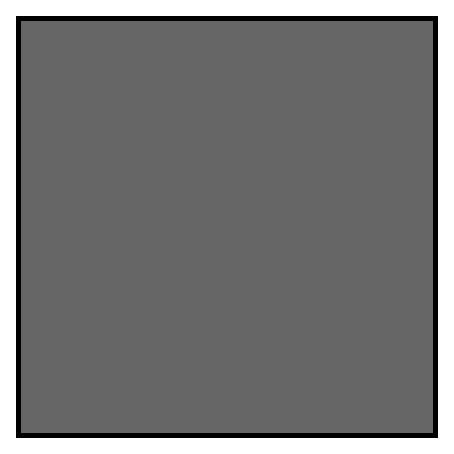
\includegraphics{example.eps}
% figure caption is below the figure
%\caption{Please write your figure caption here}
%\label{fig:1}       % Give a unique label
%\end{figure}
%
% For two-column wide figures use
%\begin{figure*}
% Use the relevant command to insert your figure file.
% For example, with the graphicx package use
 % 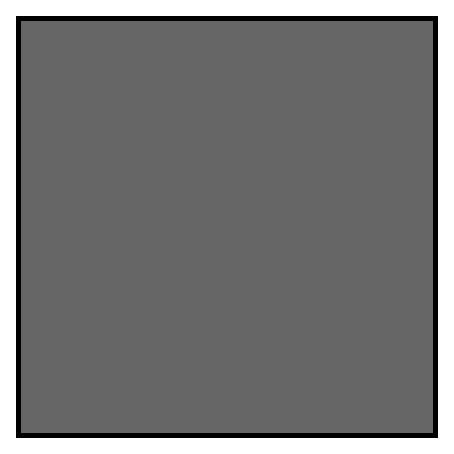
\includegraphics[width=0.75\textwidth]{example.eps}
% figure caption is below the figure
%\caption{Please write your figure caption here}
%\label{fig:2}       % Give a unique label
%\end{figure*}
%


\begin{acknowledgements}
%If you'd like to thank anyone, place your comments here
%and remove the percent signs.

\end{acknowledgements}

% BibTeX users please use one of
%\bibliographystyle{spbasic}      % basic style,
\bibliographystyle{plain}      % basic style,
% author-year citations

%\bibliographystyle{spmpsci}      % mathematics and physical sciences
%\bibliographystyle{spphys}       % APS-like style for physics
\bibliography{BibPaper2}   % name your BibTeX data base
%\printbibliography
% Non-BibTeX users please use
%\begin{thebibliography}{1}


% and use \bibitem to create references. Consult the Instructions
% for authors for reference list style.
%
%\bibitem{pa1}
% Format for Journal Reference
%Author, Article title, Journal, Volume, page numbers (year)
% Format for books
%\bibitem{RefB}
%Author, Book title, page numbers. Publisher, place (year)
% etc
%\end{thebibliography}

\end{document}
% end of file template.tex

